\documentclass[12pt,a4paper]{ufpr}
\usepackage[portuges,brazil]{babel}
% \usepackage[portuguese,brazil]{babel}

%\usepackage[brazil]{babel}
\usepackage[latin1]{inputenc}
\usepackage{amssymb,amsmath}
\usepackage{epsfig}
\usepackage{multirow}
\usepackage{xspace}
\usepackage{url}
\usepackage{etoolbox}

\usepackage{isolatin1}
\usepackage{amssymb}
\usepackage{subfigure}
\usepackage{graphicx}
\usepackage{caption2}
\usepackage{setspace}
\usepackage{ps-macros}
% \usepackage{psfig}
\usepackage{natbib} % support the \includegraphics command and options
\usepackage{array}
\usepackage{floatrow}
\floatsetup[table]{capposition=top}

\setcounter{secnumdepth}{3}    % n - numero de niveis de subsubsection numeradas
\setcounter{tocdepth}{3}       % coloca ate o nivel n no sumario

\newcommand{\sw}{\textit{software}\xspace}
\newcommand{\Sw}{\textit{Software}\xspace}
\newcommand{\sws}{\textit{softwares}\xspace}
\newcommand{\iso}{ISO/IEC 29110\xspace}
\newcommand{\gp}{Ger\^encia de Projetos\xspace}
\newcommand{\dsw}{Desenvolvimento de \Sw}
\newcommand{\bline}{\textit{baseline}\xspace}

% nomenclaturas de documenta\c{c}\~ao
\newcommand{\dt}{Declara\c{c}\~ao de Trabalho\xspace}
\newcommand{\swcfg}{Configura\c{c}\~ao de \Sw}
\newcommand{\ppj}{Plano de Projeto\xspace}
\newcommand{\prog}{Registro de Status de Progresso\xspace}
\newcommand{\qsw}{Garantia da Qualidade de \Sw}
\newcommand{\req}{Especifica\c{c}\~ao de Requisitos\xspace}
\newcommand{\aceite}{Registro de Aceite\xspace}
\newcommand{\muda}{Solicita\c{c}\~ao de Mudan\c{c}as\xspace}
\newcommand{\vcs}{Estrat\'egia de Controle de Versionamento\xspace}
\newcommand{\comp}{Componentes de \Sw}
\newcommand{\tcase}{Casos de Teste\xspace}
\newcommand{\tproc}{Procedimentos de Teste\xspace}
\newcommand{\trep}{Relat\'orio de Testes\xspace}
\newcommand{\rep}{Reposit\'orio do Projeto\xspace}
\newcommand{\vvres}{Resultados de Verifica\c{c}\~ao/Valida\c{c}\~ao\xspace}
\newcommand{\corre}{Registro de Corre\c{c}\~aes\xspace}
\newcommand{\entrega}{Instru\c{c}\~oes de Entrega\xspace}
\newcommand{\crono}{Cronograma das Tarefas do Projeto\xspace}

\newcommand{\figsource}[1]{\floatfoot{Fonte: #1}}

\title{M\'etodo de auto diagn\'ostico para implanta\c{c}\~ao da \iso}
\author{Gladistone Moreira Afonso}
\advisortitle{Orientador}
\advisorname{Prof. Dr. Ant\^onio Roberto Mury}
\advisorplace{Laborat\'orio Nacional de Computa\caption{c}\~ao Cient\'ifica, LNCC}

\city{Petr\'opolis}
\year{2015}

%\banca        % nao insira o nome do orientador, ja eh feito automaticamente
%{Prof. Dr. Antnio Roberto Mury}{Laboratrio Nacional de Computao Cientfica, LNCC}
%{Prof. Dr. Bruno Schulze}{Laboratrio Nacional de Computao Cientfica, LNCC}
%{Prof. Dr. ???}{Departamento de Informtica, UFPR} % se nao houver deixe em branco {}{}
%{Prof. Dr. ???}{Laboratrio Nacional de Computao Cientfica, LNCC}    % se houver um quarto membro na banca, inserir nome e instituicao

\defesa{ 2015 } % dia em que foi realizada a defesa da dissertacao

\newtoggle{full}
\toggletrue{full}
%\togglefalse{full}

\begin{document}

\makecapaproposta             % cria capa para proposta%

\iftoggle{full}
{
	\makecapadissertacao           % cria capa para dissertacao de mestrado %
	\makerosto                     % cria folha de rosto para versao final da UFPR %
	%\maketermo                     % cria folha com o termo de aprovacao da dissertacao%
}

%\singlespacing           % espacamento 1 - capa UFPR%
%\onehalfspacing          % espacamento 1/2 %
\doublespacing            % espacamento 2 - UFPR %

\pagestyle{headings}
\pagenumbering{roman}

% % %\chapter*{Agradecimentos}
Agrade�o primeiramente a Deus pela vida e por colocar as pessoas certas nas horas em que mais precisava para alcan�ar o sonho do Mestrado, � minha fam�lia, em especial � minha esposa M�nica e meus filhos Daniel e J�lia, ao meu orientador Prof. Dr. Ant�nio Roberto Mury, aos professores que se tornaram mestres e amigos, aos alunos e companheiros de caminhada que em muitas horas me auxiliaram e aos amigos de longa data que vieram a ser meus professores e incentivadores no in�cio desta caminhada: Prof. Dr. Ant�nio Tadeu Azevedo Gomes e Prof. Dr. F�bio Lopes Licht.          % possiu somente o texto

\tableofcontents

\listoffigures         % se houver mais do que 3 figuras
\addcontentsline{toc}{chapter}{\MakeUppercase{Lista de Figuras}}
\newpage

\listoftables        % se houver mais do que 3 tabelas
\addcontentsline{toc}{chapter}{\MakeUppercase{Lista de Tabelas}}
\newpage

\chapter*{Resumo}
\addcontentsline{toc}{chapter}{\MakeUppercase{Resumo}}
Resumo. \\
Palavras chave: ISO 29110	.           % somente o texto
\newpage

\chapter*{Abstract}
\addcontentsline{toc}{chapter}{\MakeUppercase{Abstract}}
\chapter*{Abstract}
\addcontentsline{toc}{chapter}{\MakeUppercase{Abstract}}

(vers�o do resumo em l�ngua estrangeira)

Keywords:

\newpage        % somente o texto
\newpage

\pagenumbering{arabic}

% !TEX root = dissertacao.tex
\chapter{Introdu��o}
\label{Introducao}


Esta disserta��o decidiu recorrer � problemas reais que ocorrem com grande frequ�ncia em empresas de pequeno e m�dio porte no segmento de desenvolvimento de \sw. A fim de ratificar os resultados, foi selecionada uma empresa real onde a pesquisa foi realizada.

A engenharia de \sw � um conjunto de processos com o intuito de gerar um produto final (aplicativou ou \sw) que atenda a determinada necessidade de neg�cio ou resolva determinado problema do mundo real. Sua import�ncia crece a cada dia, visto que computadores e aplicativos n�o s�o mais privil�gios �nicos de organiza��es ou de pessoas que se encaixem em classes sociais mais altas. Atualmente, aplicativos populam cada vez mais dispositivos m�veis, que por sua vez est�o cada vez mais presentes nas vidas das pessoas. Ademais, aplicativos podem ser invis�veis, presentes em dispositivos que controlam eletrodom�sticos, autom�veis entre outras m�quinas e equipamentos. � poss�vel afirmar que a engenharia de \sw permeia, de alguma forma, todas as atividades do mundo em que vivemos.

Gerenciar projetos de desenvolvimento de \sw pode se tornar uma tarefa �rdua e com diversas armadilhas caso n�o se forne�a a devida aten��o aos seus pontos cr�ticos. Como cita \cite{pressman}, a constru��o de \sw dentro de prazos estabelecidos e com qualidade ainda � um problema que atinge grande parte das empresas desenvolvedoras. Este problema tem como principal origem a falta de processos formais em alguns dos pontos cr�ticos do desenvolvimento de \sw, tais como: levantamento de requisitos, gerenciamento das mudan�as e gerenciamento das entregas \citep{martinsgerenciando}.
 
A falta de processos formais e bem definidos se mostrou mais impactante em uma das �reas-chave do neg�cio de uma empresa de desenvolvimento de \sw: a comunica��o com o cliente. Por muitas vezes os clientes n�o s�o posicionados sobre o andamento de solicita��es, prazos e custos. Tamb�m n�o h� rastreabilidade entre contatos realizados, pend�ncias geradas e tarefas agendadas. Para que se possa manter uma empresa competitiva � necess�rio atacar este problema e realizar diversas melhorias nos seus processos operacionais.
 
Um projeto de melhoria dos processos que tivesse como foco a comunica��o com o cliente iria impactar n�o somente o setor de desenvolvimento de \sw, mas todos os demais setores, disseminando a valoriza��o do cliente com um dos principais valores da empresa. Para tanto, seria necess�rio padronizar os processos dentro da organiza��o.

A escolha de padronizar os processos poderia n�o ser a �nica solu��o para os problemas encontrados, mas com certeza seria o primeiro e talvez mais portante passo para se alcan�ar a melhoria desejada. Conforme afirma \cite{toyota}, � imposs�vel melhorar qualquer processo at� que ele tenha sido padronizado.

A melhor forma de padronizar processos dentro de uma organiza��o � a ado��o de boas pr�ticas j� consagradas no mercado. Decidiu-se pela aplica��o de um conjunto de normas t�cnicas, que s�o um conjunto de documentos que estabelecem requisitos de qualidade, requisitos de desempenho, requisitos de seguran�a, processos, procedimentos, formas, dimens�es, classifica��es ou terminologias e gloss�rios \citep{normas}.

A norma escolhida, chamada de \iso, se mostrou mais pr�xima da realidade de uma pequena empresa de \sw. Esta norma, que ser� melhor detalhada no Cap�tulo \ref{Sec:iso}, foi desenvolvida especificamente para pequenas empresas ou pequenas equipes de desenvolvimento de \sw, chamadas em ingl�s de \textit{Very Small Entities} (VSE). 

A empresa alvo desta disserta��o, onde a pesquisa foi desenvolvida e aplicada e que ser� melhor detalhada no Cap�tulo \ref{sec:def:prob}, apresentou os problemas citados anteriormente. A empresa passou por um diagn�stico empresarial, melhor detalhado no Cap�tulo \ref{Sec:analise:org}, que gerou uma matriz SWOT\footnotemark{} que apontou que ela est� em franca ascens�o em termos de quantidade de novos clientes, mas os processos internos, inclusive os de desenvolvimento de \sw, n�o est�o bem formalizados para suportar este crescimento. 

\footnotetext{Avalia��o das for�as, fraquezas, oportunidades e amea�as, dos termos em ingl�s \textit{strengths, weaknesses, opportunities e threats} \citep{kotler}}

%Um dos pontos cr�ticos observados no diagn�stico foi que A falta de processos formais e bem definidos se mostrou mais impactante em uma das �reas-chave do neg�cio: a comunica��o com o cliente. Por muitas vezes os clientes n�o s�o posicionados sobre o andamento de solicita��es, prazos e custos. Tamb�m n�o h� rastreabilidade entre contatos realizados, pend�ncias geradas e tarefas agendadas. Como cita \cite{pressman}, a constru��o de \sw dentro de prazos estabelecidos e com qualidade ainda � um problema que atinge grande parte das empresas desenvolvedoras. Para que se pudesse manter a empresa competitiva era necess�rio atacar este problema e realizar algumas melhorias nos seus processos operacionais.

Este problema foi endere�ado anteriormente atrav�s da norma \iso, visto que seus processos se adequam �s necessidades da empresa foco. Algumas tentativas de implanta��o desta norma foram realizadas utilizando o aux�lio de consultores especializados mas, infelizmente, todas as tentativas foram infrut�feras e causaram grande frustra��o em todos os membros da equipe envolvidos no processo. O maior complicador que impedia a execu��o das melhorias era por onde come�ar o trabalho necess�rio para colocar a empresa no rumo correto, visto que o volume e complexidade das atividades que compunham o projeto de melhoria era muito grande, principalmente para uma empresa pequena e com recursos limitados.

\section{Defini��o do Problema}
\label{Sec:intro:problema}

Os motivos que levaram � paralisa��o e posterior abandono da implanta��o da \iso foram a grande quantidade de processos novos que deveriam ser criados ou processos antigos que deveriam ser revisados. O esfor�o necess�rio para levar a empresa da situa��o atual para a situa��o desejada era muito grande. Os custos financeiros, operacionais e de recursos, principalmente para se iniciar o projeto de melhorias, contrastava com os riscos eminentes de qualquer projeto dessa magnitude: fracasso e perda dos investimentos.

Seria necess�rio diminuir as probabilidades destes riscos ocorrerem para que o projeto de melhoria se tornasse mais atrativo para a empresa, apesar da ci�ncia da alta diretoria e dos demais membros da equipe da import�ncia estrat�gica de um conjunto de processos bem definidos e alinhados com os valores da empresa.

Nenhum m�todo preexistente e nem mesmo os consultores especializados na implanta��o da \iso conseguiram suplantar essa dificuldade encontrada pela empresa. Para suprir esta lacuna, esta disserta��o objetiva a cria��o de um m�todo que contemple ferramentas capazes de auxiliar uma empresa na implanta��o da \iso, permitindo que esta possa selecionar a melhor forma de iniciar o projeto e, com isso, aumentar a motiva��o da equipe e diminuir os riscos de paralisa��o e abandono do projeto. 

Os resultados aqui alcan�ados dever�o ser amplos o suficiente para auxiliar outras empresas com os mesmos problemas e at� mesmo consultores e especialistas na norma \iso, que poder�o utilizas as ferramentas desenvolvidas nos seus diagn�sticos.

\section{Delimita��o do Trabalho}
\label{Sec:delim:trab}

Para possibilitar uma implanta��o gradativa e que traga resultados mais relevantes em suas primeiras etapas, a proposta desta disserta��o � criar um m�todo de auto diagn�stico que leve em considera��o os valores individuais de cada empresa e que permita classificar as etapas iniciais de implanta��o da \iso de acordo com esses valores. Um dos principais benef�cios esperados deste m�todo � que a equipe se mantenha motivada ao perceber as vantagens da utiliza��o da \iso nos est�gios iniciais, impedindo o abandono prematuro da implanta��o das melhorias e o consequente abandono do projeto. 

Este trabalho, por�m, n�o contempla a an�lise do projeto de implanta��o das melhorias. Somente ser�o analisados qualitativamente os resultados do m�todo de auto diagn�stico.

Portanto, este trabalho de disserta��o tem como objetivo \textbf{criar um m�todo de auto diagn�stico para implanta��o da \iso que priorize processos com maior ader�ncia aos valores individuais de cada empresa e que tragam benef�cios relevantes observ�veis nas etapas iniciais da implanta��o}.
	
\section{Organiza��o do Trabalho}

Este trabalho est� organizado da seguinte forma: No Cap�tulo 1 � apresentada uma breve introdu��o; no Cap�tulo 2 s�o apresentadas as revis�es bibliogr�ficas, as tecnologias envolvidas, os trabalhos relacionados e os conceitos b�sicos necess�rios ao entendimento dos cap�tulos seguintes; no Cap�tulo 3 � apresentada a descri��o da proposta e a metodologia utilizada para a obten��o dos resultados; no Cap�tulo 4 s�o apresentados os resultados obtidos; no Cap�tulo 5 s�o analisados os resultados obtidos e no Cap�tulo 6 s�o apresentadas as conclus�es e os trabalhos futuros.
% !TEX root = dissertacao.tex
\chapter{Revis�o Bibliogr�fica}
\label{tecnologias}

Este capt�ulo apresenta ao leitor as principais tecnologias envolvidas no trabalho, os conceitos e defini��es dos termos utilizados na disserta��o.

\section{Engenharia de \sw}

De acordo com \cite{pressman}, a engenharia de \sw � uma tecnologia em camadas e qualquer abordagem de engenharia deve se apoiar em um compromisso organizacional com a \textbf{qualidade} e com um processo cont�nuo de aperfei�oamento, como ilustrado na Figura \ref{fig:sw.camadas}. Algumas ferramentas da administra��o e filosofias, tais como Gest�o da Qualidade Total\footnotemark \footnotetext{\textit{Total Quality Management} (TQM) consiste numa estrat�gia de administra��o orientada a criar consci�ncia da qualidade em todos os processos organizacionais.}, Seis Sigma\footnotemark \footnotetext{\textit{Six Sigma} � um conjunto de pr�ticas originalmente desenvolvidas pela Motorola para melhorar sistematicamente os processos ao eliminar defeitos.} e Manufatura Enxuta\footnotemark, podem instituir a cultura de qualidade necess�ria para esta ind�stria.

\footnotetext{\textit{Lean Manufacturing} ou Sistema Toyota de Produ��o � uma filosofia de gest�o focada na redu��o de desperd�cios.}

\begin{figure}[!h]
\centering
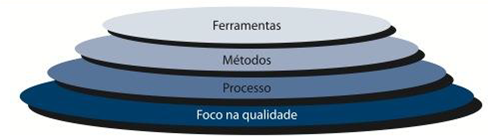
\includegraphics[scale=1]{figuras/eng_sw_camadas.png}
\caption{Camadas da engenharia de \sw \cite[p.17]{pressman}}
%http://www.devmedia.com.br/principios-da-engenharia-de-software/29630
\label{fig:sw.camadas}
\end{figure}

As pr�xima camada, \textbf{processo}, define regras e padr�es que permitem o controle e ger�ncia dos projetos de desenvolvimento, al�m de estabelecer o contexto no qual as pr�ximas camadas ir�o atuar. Os \textbf{m�todos} oferecem t�cnicas de constru��o dos \sws (como fazer) e as \textbf{ferramentas} fornecem apoio para as primeiras camadas e podem ser automatizadas ou semi-automatizadas, integradas ou n�o, gratuitas ou pagas, etc.

Alguns problemas antigos da engenharia de \sw, que teve seu in�cio na d�cada de 50, ainda convivem com as empresas desenvolvedores nos dias atuais: precariedade  nas  previs�es  e  planejamentos, baixa qualidade de processos e produtos, requisitos  mal  definidos e o alto custo para manuten��o. Tais problemas podem ser atribu�dos � gest�o ineficiente ou inadequada dos projetos e consomem recursos importantes (humanos e financeiros, principalmente) por conta do retrabalho.

\section{\iso}
\label{Sec:iso}

\subsection{Representatitividade e dificuldades das VSEs}

A ind�stria de \sw representa 8\% do PIB e 6\% dos postos de trabalho na Europa e pequenas e m�dias empresas de desenvolvimento respondem por 90\% dos neg�cios formais que geram entre 40\% e 50\% do total de empregos \cite{reicis}. Empresas com 10 ou menos funcion�rios representam 85\% do total na Europa e 50\% em Montreal, Canad�, considerando somente empresas de TI e 93\% na Europa e 50\% nos Estados Unidos, considerando qualquer tipo de empresa \cite{ieee_comp}. 

O Brasil, que em 2011 passou a ocupar a 10\textsuperscript{a} posi��o no \textit{ranking} mundial de \sw e servi�os com um faturamento de cerca de US\$ 21 bilh�es de d�lares, possui 97,3\% das quase 70 mil empresas do setor classificadas como Micro e Pequeno Empresas (MPE) com at� 19 pessoas \cite{guia.sebrae}.

Apesar de representativas, estudos apontam que estas pequenas e m�dias empresas de \sw n�o s�o atendidas por normas e padr�es que se encaixem em suas realidades. Padr�es internacionais, como ISO e IEEE, apresentam diversas barreiras econ�micas e operacionais que tornam virtualmente imposs�vel a sua implementa��o por uma VSE.

De acordo com \cite{fayad}, existem quatro quest�es que n�o s�o tratadas de forma adequada pela literatura na �rea de engenharia de \sw:

\begin{itemize}

\item \textbf{Tamanho da empresa}: ind�stria, governo, associa��es e outras institui��es podem definir n�meros diferentes para designar que uma empresa � pequena, podendo variar de 10 a 500 funcion�rios ou mais. Al�m disso, empresas que n�o possuem foco somente no desenvolvimento de \sw podem possuir um contingente muito grande de funcion�rios, por�m somente um pequeno percentual deste total dedicado �s atividades de \sw.

\item \textbf{Modo de desenvolvimento}: o modelo de contrato sugerido pela literatura, onde o cliente do \sw � identificado, mesmo que seja um departamento dentro de uma empresa, nem sempre funciona para pequenas empresas. Estas, geralmente, n�o se utilizam de contratos formais, n�o conseguem identificar ou isolar bem o cliente ou simplesmente os profissionais de TI n�o ``perdem tempo'' com isso porque precisam manter o foco nas especifica��es do produto.

\item \textbf{Velocidade de desenvolvimento}: competitividade acirrada e demanda de entregas r�pidas pelo mercado frutificaram em novas estrat�gias r�pidas de desenvolvimento.
 
\item \textbf{Tamanho de desenvolvimento}: hoje o n�mero de linhas de c�digo dos \sws considerados pequenos supera o n�mero de linhas dos \sws considerados grandes no passado. Isso incorre no fato que pequenas empresas come�am a necessitar de metodologias de \sw desenvolvidas para projetos de larga escala que, infelizmente, n�o se apadtam bem aos projetos de pequena escala.
 
\end{itemize}

Como tentativa de contornar as principais barreiras e tratar de melhor forma as quest�es citadas acima, algumas propostas de melhoria dos processos de desenvolvimento de \sw foram adotados ao redor do mundo, sendos os principais:

\begin{itemize}

\item \textbf{SPIRE\footnotemark e TOPS\footnotemark} promovidos pela Uni�o Europeia atrav�s do \textit{European Software and System Initiative} (ESSI);

\item \textbf{MoProSoft} adotado pelo M�xico para a ind�stria de \sw, baseado na ISO 12207, CMM e ISO 9001;

\item \textbf{EvalProSoft} tamb�m adotado pelo M�xico, baseado na ISO 15504;

\item \textbf{MPS-BR} no Brasil tem como m�todo de avalia��o o MA-MPS, baseado na ISO 15504;

\item \textbf{COMPETISOFT} estabelecido na Iberoam�rica, que tem seu modelo de refer�ncia baseado na ISO 12207, CMM, ISO 9001, MANTEMA  e m�trica V3, seu m�todo de avalia��o sugerido baseado na ISO 15504 e seu modelo de gest�o de melhora influenciado pelo IDEAL e SCRUM;

\item \textbf{IPRC} � o Cons�rcio Internacional de Investiga��o de Processos criado pelo SEI com o objetivo de melhorar processos para os chamados \textit{Small Settings} (IPSS), referentes aos projetos com menos de 20 pessoas, organiza��es com menos de 50 pessoas e/ou empresas com menos de 100 pessoas;

\item \textbf{I.T.Mark} foi desenvolvido e aplicado na Europa, �sia e Iberoam�rica pelo ESI e se baseia no CMMI e ISO 17799:2005.

\end{itemize}

\footnotetext[1]{\url{http://www.cse.dcu.ie/spire/}} 

\footnotetext{\url{http://cordis.europa.eu/esprit/src/27977.htm}} 

\subsection{Hist�ria da \iso}

Em 2004, durante a reuni�o plen�ria do SC7\footnotemark{} na Austr�lia, delegados de cinco na��es chegaram a um consenso a respeito da necessidade da cria��o de padr�es internacionais que atendessem ao tamanho e particularidades das VSEs. Os padr�es deveriam incluir perfis e guias e o grupo chegou a um acordo sobre os seguintes objetivos gerais:

\footnotetext{ISO/IEC JTC 1/SC 7 \textit{Software and systems engineering} -  \url{http://www.iso.org/iso/iso_technical_committee?commid=45086}}

\begin{itemize}

\item Fazer com que os padr�es atuais de engenharia de \sw fossem mais acess�veis �s VSEs;

\item Fornecer documenta��es que requeiram o m�nimo de esfor�o em adapta��es;

\item Fornecer documenta��es harmonizadas integrando padr�es j� dispon�veis como padr�es de processos, produtos de trabalho e entreg�veis, ferramentas de avalia��es, qualidade e modelagem;

\item Levar em considera��o, se desej�vel, as no��es de n�veis de capacidade e maturidade apresentados na ISO/IEC 15504 e no CMMI.

\end{itemize}

Em 2005, na reuni�o plen�ria do SC7 na Finl�ndia, a Tail�ndia prop�s a cria��o de um grupo de trabalhos para atingir estes objetivos, que foi aprovada por doze pa�ses e estabeleceu o \textit{Working Group} 24 (WG24) com os seguintes pa�ses membros: B�lgica, Canad�, Rep�blica Tcheca, Irlanda, It�lia, Jap�o, Cor�ia, Luxemburgo, �frica do Sul, Tail�ndia, Reino Unido e os Estados Unidos.

Uma pesquisa foi conduzida pelo WG24 para refinar os requisitos das VSEs e estas foram questionadas sobre a sua utiliza��o dos padr�es ISO/SC7 e tamb�m sobre problemas e poss�veis solu��es que poderiam ajudar na aplica��o de padr�es e torn�-las mais competitivas. O Brasil foi o pa�s com o segundo maior n�mero de respostas, totalizando 68, perdendo somente para a Col�mbia, com 88. O objetivo desta pesquisa foi validar algumas hip�teses, incluindo:

\begin{itemize}

\item O contexto das VSEs requer perfis de ciclo de vida leves e muito bem focados;

\item Contextos de neg�cio particulares requerem perfis particulares;

\item Existem diferen�as significantes em termos de recursos e infraestrutura dispon�veis entre uma VSE que emprega de 1 a 10 pessoas e um departamento de TI do mesmo tamanho em uma empresa grande;

\item As VSEs s�o limitadas em tempo e recursos, o que leva a uma falta de entendimento sobre como os uso dos padr�es podem benefici�-las;

\item Os benef�cios para VSEs podem incluir reconhecimento atrav�s de avaliac�es ou auditorias realizadas por um �rg�o acreditado.

\end{itemize}

A pesquisa incluiu propositalmente questionamentos sobre o porqu� da pouca ado��o de padr�es e descobriu-se que eram tr�s os principais motivos: 

\begin{itemize}

\item Falta de recursos - 28\%;

\item N�o eram necess�rios - 24\%;

\item A natureza em si dos padr�es - 15\% (consideravam os padr�es dif�ceis e burocr�ticos e n�o forneciam acompanhamento adequado para uso em pequenos ambientes empresariais).

\end{itemize}

Apesar disso, uma maioria de tr�s quartos achavam importante serem avaliadas ou certificadas em um padr�o, sendo a certifica��o ISO mencionada por 40\% dos entrevistados. A procura por reconhecimento oficial de mercado foi citada por 28\% das empresas e, destas, somente 4\% estavam interessadas em uma certifica��o nacional. Os principais benef�cios que uma certifica��o poderia trazer inclu�am:

\begin{itemize}

\item Aumento na competitividade;

\item Maior satisfa��o e confian�a dos clientes;

\item Maior qualidade de produto de \sw;

\item Aumento no patroc�nio para melhoria de processos;

\item Redu��o nos riscos de desenvolvimento;

\item Facilita��o de marketing;

\item Maior potencial para exporta��o.

\end{itemize}

A pesquisa tambem apontou que as VSEs requerem assist�ncia, guias com exemplos e padr�es leves e f�ceis de entendimento, com modelos (\textit{templates}) completos. Houve a indica��o de que � possivel implementar padr�es com um m�nimo de custo, tempo e recursos.

A abordagem do WG24 foi utilizar o conceito de perfis da ISO, ou \textit{International Standardized Profile} (ISP), para desenvolver os novos padr�es para VSEs. Os perfis s�o formados por um conjunto de padr�es e/ou ISPs, b�sicos ou modificados, necess�rios para se atingir uma fun��o particular. As modifica��es podem se dar na forma da escolha de classes, subconjuntos conformes, op��es e par�metros dos perfis e ISPs b�sicos.

Inicialmente o WG24 procurou por padr�es existentes para customizar de acordo com as necessidades das VSEs, sendo o padr�o mexicano para desenvolvimento de \sw (Moprosoft) o primeiro selecionado. Este padr�o tem a ISO/IEC 12207 como base e pega emprestado pr�ticas principalmente da ISO9001, CMMI e PMBOK. Posteriormente identificou-se que este padr�o atendia empresas maiores que as VSEs alvo e algumas modifica��es foram feitas para adequ�-lo ao n�mero de funcion�rios, em duas fases distintas: 1) menos de 10 funcion�rios e 2) 10 a 25 funcion�rios.

Os primeiros perfis continham basicamente tarefas vindas da ger�ncia de projetos e processos de desenvolvimento de \sw, atividades consideradas como chave para uma VSE. Posteriormente foram definidos guias explicando em mais detalhes os processos definidos no perfil, publicados em relat�rios t�cnicos que deveriam ser disponibilizados gratuitamente para as VSEs. Os guias cont�m uma s�rie de pacotes de implantac�o (\textit{deployment packages}) contendo um conjunto de artefatos desenvolvidos para facilitar e acelerar a implementa��o de uma s�rie de pr�ticas. Cada pacote de implanta��o inclui, tipicamente, a descri��o do processo (tarefas, entradas, sa�das e pap�is), guia, modelo, checklist, exemplo, material de apresenta��o, mapeamento para padr�es e modelos, e uma lista de ferramentas para auxiliar VSEs a implementar o processo.

\subsection{Benef�cios da \iso}

A utiliza��o da \iso pode beneficiar empreendimentos cujo tamanho levaria ao descarte imediato de padr�es e metodologias, por serem considerados burocr�ticos, caros e impratic�veis para pequenas empresas. O artigo de \cite{swicetrip} mostra que � possivel aplicar o padr�o e obter resultados excelentes para um empreendimento composto de somente duas pessoas.

Ao aplicar os conceitos e ferramentas disponibilizadas pela \iso, uma empresa poder� ter controle sobre:

\begin{itemize}

\item  \textbf{Escopo:} saber o que est� sendo feito e por qu�, al�m de determinar se  o \sw faz o que deveria fazer tecnicamente e atende aos requisitos do cliente;

\item  \textbf{Prazo e or�amento:} varia��es s�o controladas e a empresa � capaz de determinar quando o projeto acaba e se inicia a fase de manuten��o;

\item  \textbf{Integra��o:} todos da equipe tem o mesmo entendimento sobre o projeto e a empresa consegue integrar o que duas ou mais pessoas est�o produzindo;

\item  \textbf{Mudan�as:} todos est�o cientes que ela vai ocorrer e est�o preparados para conhecer seus impactos e incorpor�-las ao trabalhao de forma adequada;

\item  \textbf{Demanda:} a empresa estar� pronta para o seu aumento, tanto de clientes como de produtos.

\end{itemize}

Como consequ�ncia direta dos itens citados anteriormente, a empresa de \sw passa a ter maior credibilidade no mercado. Sua capacidade de produzir mais r�pido e reagir melhor �s mudan�as se refletem na melhora da qualidade e aumento da competitividade. Caso opte pela certifica��o, ainda poder� contar com o todo o reconhecimento internacional que a institui��o ISO oferece e ter sua entrada no mercado internacional facilitada.

\subsection{Divis�o da \iso}

A \iso � dividida em cinco partes, sendo uma vis�o global, dois perfis (\textit{Framework} e taxonomia e especifica��es de perfis das VSE) e dois guias (guia de avalia��o e guia de gest�o e engenharia). Sua composi��o pode ser visualizada na Figura \ref{fig:serie:iso}.

\begin{figure}[!h]
\centering
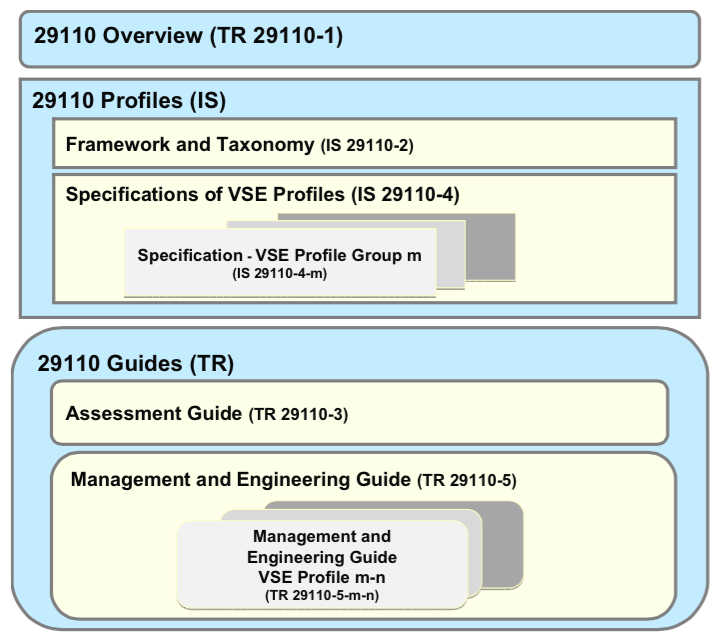
\includegraphics[scale=0.4]{figuras/serie_iso.png}
\caption{S�rie \iso \cite[p�g. 7]{iso}}
\label{fig:serie:iso}
\end{figure}

O guia de gest�o e engenharia oferece �s VSE processos de \gp e \dsw que, de acordo com \cite{iso}, fazem com que os desenvolvedores ganhem benef�cios atrav�s dos seguintes aspectos alcan�ados:

\begin{itemize}

\item Um conjunto de requisitos de projeto e produtos esperados � entregue ao cliente;

\item Um processo disciplinado de gest�o que oferece visibilidade do projeto e a��es corretivas para problemas e desvios de projeto � realizado;

\item Um processo sistem�tico e disciplinado de desenvolvimento de \sw que satisfa�a as necessidades do cliente e assegure a qualidade do produto � seguido.

\end{itemize}

O guia tamb�m cita algumas condi��es iniciais para que a VSE possa utiliz�-lo \cite{iso}:

\begin{itemize}

\item Documenta��o da Declara��o de Trabalho do projeto;

\item Realiza��o do estudo de viabilidade do projeto, antes do seu in�cio;

\item Atribui��o e treinamento da equipe de projeto, incluindo o gerente de projeto;

\item Disponibilidade de bens, servi�os e infraestrutura para se iniciar o projeto.

\end{itemize}

Os processos de \gp e \dsw s�o interrelacionados, sendo a entrada do primeiro a \dt e sa�da do �ltimo a \swcfg, conforme pode ser observado na Figura \ref{fig:gp:dsw}. 

A \gp est� ligada ao estabelecimento e controle das tarefas para se alcan�ar os objetivos do projeto em termos de qualidade, tempo e custo. O \dsw est� relacionado �s atividades de constru��o, integra��o e testes de \sw.

\begin{figure}[!h]
\centering
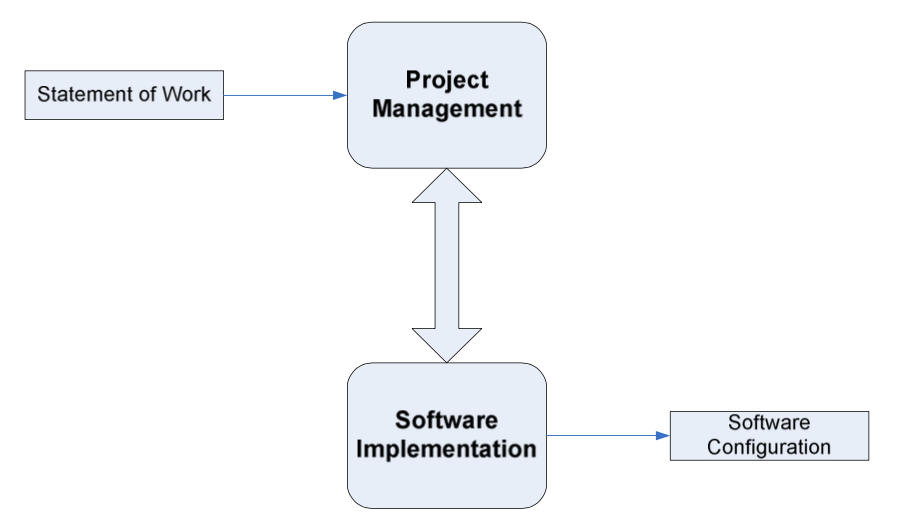
\includegraphics[scale=0.3]{figuras/gp_desenv_sw.png}
\caption{Processos b�sicos \cite[p�g. 12]{iso}}
\label{fig:gp:dsw}
\end{figure}

\subsection{\gp}
\label{Sec:iso:obj:gp}

De acordo com \cite{iso}, os objetivos deste processo s�o:

\begin{itemize}

\item[PM.O1] O \ppj � desenvolvido de acordo com a \dt e � revisado e aceito pelo cliente. As tarefas e recursos necess�rios para completar o trabalho s�o quantificados e estimados.

\item[PM.02] O progresso do projeto � monitorado em rela��o ao \ppj e registrado no \prog. Corre��es para remediar problemas e desvios do plano s�o tomadas quando os objetivos do projeto n�o s�o alcan�ados. O fechamento do projeto � realizado para se conseguir o aceite do cliente documentado no \aceite.

\item[PM.03] A \muda � abordada atrav�s de sua recep��o e an�lise. Mudan�as aos requisitos de \sw s�o avaliadas em custo, cronograma e impacto t�cnico.

\item[PM.O4] Reuni�es de revis�o s�o realizadas com a equipe de trabalho e o cliente. Acertos s�o registrados e rastreados.

\item[PM.O5] Riscos s�o identificados conforme aparecem e durante a condu��o do projeto.

\item[PM.O6] Uma \vcs de \sw � desenvolvida. Itens da \swcfg s�o identificados, definidos e inclu�dos em uma \bline. Modifica��es e entregas de um item s�o controladas e disponibilizadas ao cliente e equipe de trabalho. O armazenamento, manuseio e entrega dos itens s�o controlados.

\item[PM.O7] A \qsw � realizada para garantir que os produtos de trabalho e processos obede�am ao \ppj e \req.

\end{itemize}

Cada um destes objetivos pode ser alcan�ado atrav�s de uma s�rie de processos que, por sua vez, ir�o gerar v�rios documentos de apoio. Os processos e o fluxo de informa��o que percorre estes processos podem ser resumidos na Figura \ref{fig:gp:diagr}.

\begin{figure}[!h]
\centering
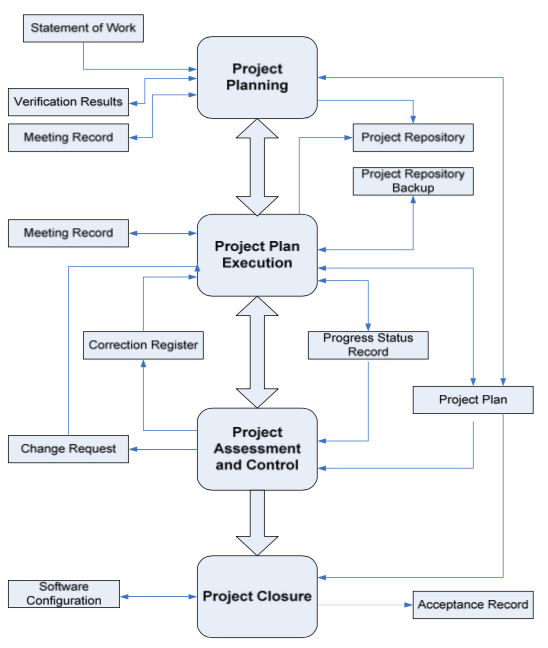
\includegraphics[scale=0.5]{figuras/gp_diagr.png}
\caption{Diagrama do processo de \gp \cite[p�g. 12]{iso}}
\label{fig:gp:diagr}
\end{figure}

\subsection{\dsw}
\label{Sec:iso:obj:dsw}

De acordo com \cite{iso}, os objetivos deste processo s�o:

\begin{itemize}

\item[SI.O1] As tarefas das atividades s�o feitas atrav�s da realiza��o do \ppj corrente.

\item[SI.02] Os requisitos de \sw s�o definidos, analisados para corre��o e testabilidade, aprovados pelo cliente, inclu�dos na \bline e comunicados.

\item[SI.03] O projeto de \sw, com arquitetura e detalhamento, � desenvolvido e inclu�do na \bline. Ele descreve os \comp e suas interfaces internas e externas. A consist�ncia e rastreabilidade aos requisitos de \sw s�o estabelecidas.

\item[SI.O4] \comp definidos pelo projeto s�o produzidos. Testes unit�rios s�o definidos e realizados para verificar a consist�ncia com os requisitos e o projeto. Rastreabilidade com os requisitos e projeto s�o estabelecidos.

\item[SI.O5] \Sw � produzido atrav�s da integra��o de \comp e verificados usando \tcase e \tproc. Resultados s�o registrados no \trep. Defeitos s�o corrigidos e a consist�ncia e rastreabilidade com o projeto de \sw s�o estabelecidos.

\item[SI.O6] Uma \swcfg, que cumpra com o \req acertado com o cliente, que inclua documenta��es de usu�rio, opera��o e manuten��o � integrada, inclu�da na \bline e armazenada no \rep. Necessidades de mudan�a na \swcfg s�o detectadas e os pedidos de mudan�a relacionados s�o iniciados.

\item[SI.O7] Tarefas de valida��o e verifica��o de todos os produtos de trabalho requeridos s�o realizadas usando os crit�rios definidos para se alcan�ar a consist�ncia entre produtos de sa�da e entrada em cada atividade. Defeitos s�o identificados e corrigidos. Registros s�o armazenados nos \vvres.

\end{itemize}

Cada um destes objetivos pode ser alcan�ado atrav�s de uma s�rie de processos que, por sua vez, ir�o gerar v�rios documentos de apoio. Os processos e o fluxo de informa��o que percorre estes processos podem ser resumidos na Figura \ref{fig:dsw:diagr}.

\begin{figure}[!h]
\centering
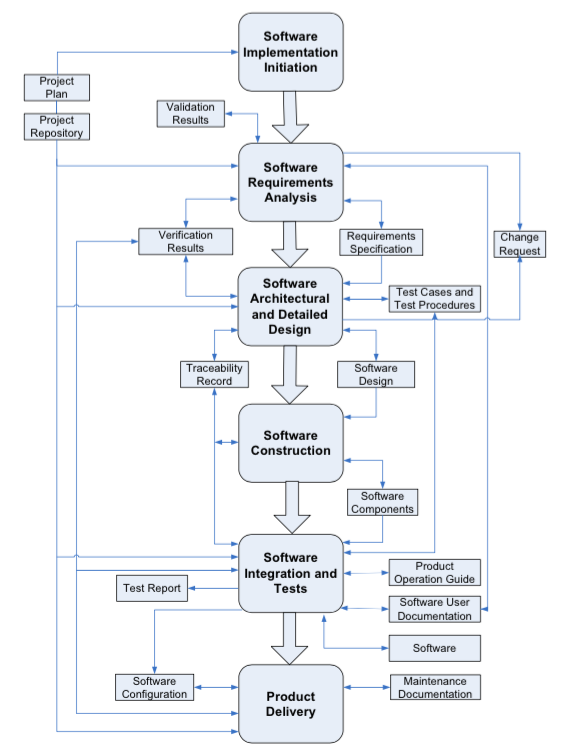
\includegraphics[scale=0.5]{figuras/dsw_diagr.png}
\caption{Diagrama do processo de \dsw \cite[p�g. 30]{iso}}
\label{fig:dsw:diagr}
\end{figure}

\section{Tecnologias Envolvidas}

%	Esta seo apresenta os principais conceitos e tecnologias utilizadas no trabalho proposto. Na Seo \ref{computacaoEmNuvem}  apresentado o conceito de computao em nuvem. As Caractersticas Essenciais de uma Nuvem so apresentadas na Seo \ref{CaracteristicasEssenciaisdeumaNuvem} e na Seo \ref{ModelosDeNuvem} so apresentados os modelos de nuvem. Na Seo \ref{ComputacaoDeAltoDesempenho} descreve-se a computao de alto desempenho e na Seo \ref{Virtualizacao} o conceito e os tipos de virtualizao. Na Seo \ref{comerciaisXcientificas} apresentam-se as principais diferenas entre aplicaes comerciais e cientficas, seguido do conceito de dependabilidade na Seo \ref{dependabilidade}. \\
	
%\subsection{Programa��o multi-plataforma}

%Vale a pena mencionar que o \sw foi pensado como multi-plataforma para facilitar a vida da empresa (se utilizar de dispositivos m�veis, n�o depender de hardware, etc)?
% !TEX root = dissertacao.tex
\chapter{Descri��o da Proposta}
\label{proposta}

Como visto no Cap�tulo \ref{Introducao}, era necess�rio encontrar uma solu��o que tornasse vi�vel a implanta��o da Norma \iso em uma pequena empresa de desenvolvimento de \sw com o menor risco poss�vel de paralisa��o e abandono nas suas fases iniciais.

Muitas empresas e especialistas em implanta��o da Norma \iso se utilizam de question�rios para realizar a avalia��o inicial do estado atual das empresas de \sw e determinar o caminho que dever� ser percorrido, atrav�s da implanta��o dos processos da Norma, para se alcan�ar o estado desejado. Por�m, estes question�rios n�o s�o disponibilizados para um auto diagn�stico e � necess�rio arcar com o alto custo da consultoria inicial para conseguir os resultados que podem demorar a ser divulgados. Ademais, os question�rios de avalia��o colocam todas as atividades e tarefas da \iso em um mesmo patamar de import�ncia, sem levar em considera��o os valores das empresas alvo. 
	
A proposta desta disserta��o � auxiliar a an�lise e a posterior cria��o de um question�rio de auto diagn�stico para implanta��o da \iso que priorize processos com maior ader�ncia aos valores individuais de cada empresa e que tragam benef�cios relevantes observ�veis nas etapas iniciais da implanta��o.

\section{Defini��o do Problema}
\label{sec:def:prob}

O primeiro passo tomado neste estudo foi formalizar a defini��o do problema e a sua delimita��o. Foi constatado que nenhum m�todo preexistente era capaz de auxiliar as empresas conforme a proposta colocada anteriormente. Para ent�o procurar cobrir essa lacuna o seguinte problema para estudo foi definido:

\begin{itemize}

\item Pequenas empresas de \sw geralmente possuem grandes limita��es de recursos financeiros, humanos e materiais para executar projetos de melhorias de processos, principalmente os que representam custos maiores como Normas ISO. Mesmo cientes dos benef�cios que podem representar, muitos empres�rios se mostram receosos em implantar essas solu��es por conta dos altos riscos de insucesso provenientes da desmotiva��o que se abate nos est�gios iniciais onde o trabalho � muito dispendioso e os benef�cios observ�veis s�o pequenos ou nulos.

\item A an�lise inicial, que determina o estado atual da empresa desenvolvedora de \sw, � realizado atrav�s de uma empresa ou consultor especializado, cujo custo pode ser muito alto, a metodologia n�o � acess�vel e os resultados podem demorar a chegar nas m�os dos clientes.

\item As a��es de corre��o e melhoria sugeridas a partir da an�lise inicial n�o levam em considera��o os valores da empresa e colocam no mesmo patamar todas as atividades e tarefas. Ao implantar uma a��o que n�o traga um benef�cio relevante, os membros da equipe podem se sentir desmotivados e o projeto fica mais sujeito a paralisa��es e um poss�vel abandono.

\end{itemize}

\section{Justificativa do Trabalho}

Este trabalho tem como justificativa principal a demanda por melhorias no processo de desenvolvimento de \sw para empresas de pequeno e m�dio porte, focando no diagn�stico da empresa alvo realizado no Ap�ndice \ref{Sec:analise:org}. 

Al�m da aplica��o imediata na empresa alvo, a ferramenta de auto diagn�stico criada a partir desta disserta��o tamb�m servir� de apoio a outras empresas de desenvolvimento de \sw que pretendam implantar a Norma \iso ou a empresas e consultores especializados que poder�o se beneficiar de uma an�lise inicial mais focada nos valores das empresas.

\section{Descri��o da empresa alvo}
\label{Sec:empresa}

A DataSerra Loca��o de Programas de Computador Ltda ME foi escolhida como empresa objeto de estudo por ter em seu quadro societ�rio o autor desta disserta��o.

A empresa foi fundada no ano de 1997, est� situada na cidade de Petr�polis, estado do Rio de Janeiro, mas possui alcance nacional, atendendo clientes em diversos outros estados. Seu segmento de atua��o � no ramo de Tecnologia da Informa��o, produzindo \sws, prestando suporte, consultoria e treinamentos, al�m de fornecer equipamentos de automa��o comercial.

A DataSerra possui 6 colaboradores, al�m dos seus dois s�cios, e seu organograma est� representado na Figura \ref{Fig:organograma}. O porte da empresa se encaixa perfeitamente na classifica��o de VSE determinada pela Norma \iso, mais detalhada na Se��o \ref{Sec:iso}.

	\begin{figure}[!h]
		\centering
		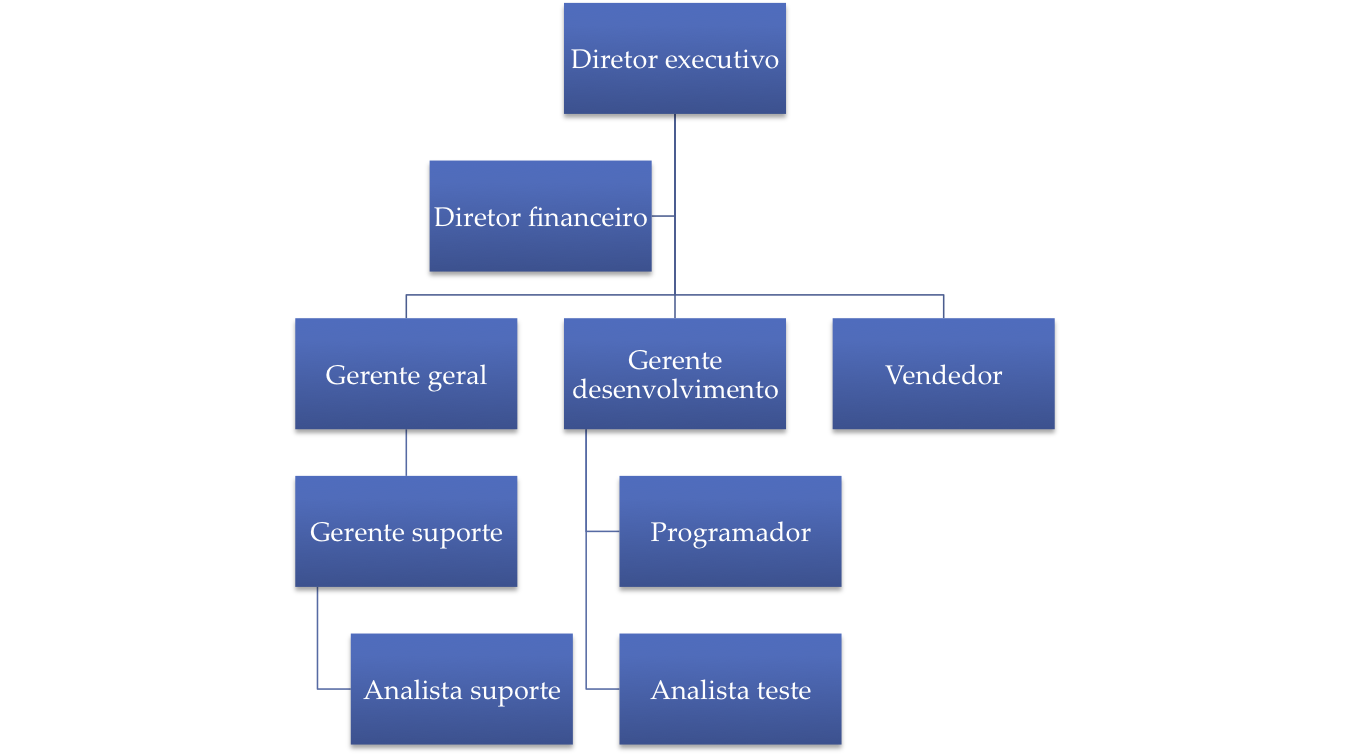
\includegraphics[scale=0.6]{figuras/organograma.png}
		\caption{Organograma da DataSerra}
		\label{Fig:organograma}
	\end{figure}
	

\section{Metodologia e Desenvolvimento}
\label{Sec:metodologia}

Esta disserta��o foi constru�da atrav�s da pesquisa bibliogr�fica e da pesquisa aplicada, ou tecnol�gica, onde se procurou resolver um problema real buscando solu��es atrav�s do m�todo cient�fico \citep{metodos}.

A metodologia deste trabalho passou pelas 4 fases do m�todo cient�fico: problema, teoria, pr�tica e divulga��o. Estas fases est�o representadas na Figura \ref{Fig:metodo:cientifico}. A fase do problema foi descrita em detalhes no Cap�tulo \ref{Introducao}. As demais fases ser�o cobertas a seguir neste Cap�tulo.

	\begin{figure}[!h]
		\centering
		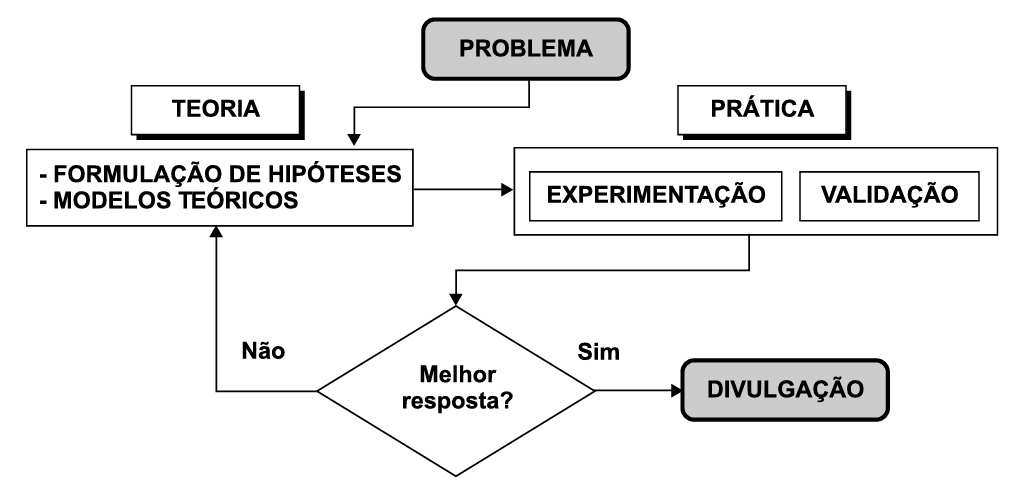
\includegraphics[scale=0.5]{figuras/metodo_cientifico.png}
		\caption{Fases do m�todo cient�fico}
		\figsource{\citealp[p. 10]{metodos}}
		\label{Fig:metodo:cientifico}
	\end{figure}

Levando em considera��o o objetivo desta disserta��o:

\begin{quote}
	``Criar um m�todo de auto diagn�stico para implanta��o da \iso que priorize processos com maior ader�ncia aos valores individuais de cada empresa e que tragam benef�cios relevantes observ�veis nas etapas iniciais da implanta��o'' (Se��o \ref{Sec:objetivo}) 
\end{quote} levantou-se como hip�tese b�sica que uma das melhores solu��es era a implanta��o de um question�rio de auto avalia��o. A fim de produzir este question�rio, foram pesquisados na literatura outros autores que houvessem passado por um problema semelhante e tivessem produzido uma ferramenta com as mesmas caracter�sticas. N�o foi poss�vel encontrar trabalhos com a mesma finalidade, mas  foi obtido sucesso em coletar algumas informa��es sobre m�todos de cria��o de pesquisas de mercado, que se utilizam de question�rios como ferramenta principal de aplica��o.

\iftoggle{full}
{
	
	Dentre os trabalhos encontrados, o artigo de \cite{manzato} define uma abordagem estat�stica para pesquisas qualitativas que foi adaptada �s necessidades desta disserta��o. Sua representa��o gr�fica pode ser observada na Figura \ref{Fig:abordagem:pesquisa}. 

	Os primeiros itens da abordagem citada anteriormente s�o a defini��o do problema, que foi tratado e bem delimitado nesta disserta��o na Se��o \ref{Sec:intro:problema}, e o planejamento amostral, que n�o foi realizado por se tratar de um question�rio individual e o p�blico alvo ser bem estratificado, composto de pequenas empresas de desenvolvimento de \sw.

	\begin{figure}[!h]
		\centering
		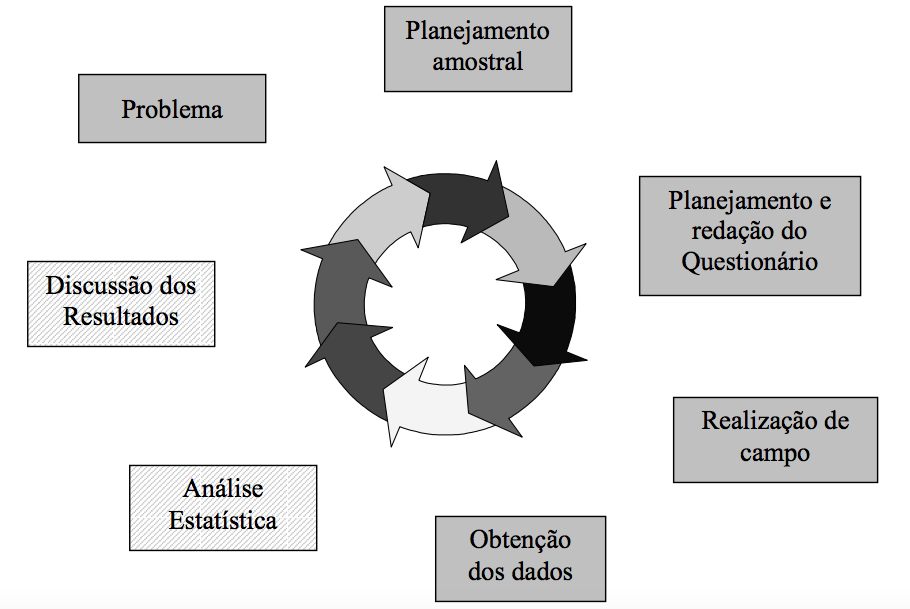
\includegraphics[scale=0.5]{figuras/abordagem_pesquisa.png}
		\caption{Abordagem estat�stica na pesquisa quantitativa}
		\figsource{\citealp{manzato}}
		\label{Fig:abordagem:pesquisa}
	\end{figure}

	O passo seguinte, planejamento do question�rio, � o ponto do processo onde esta disserta��o se diferencia dos demais trabalhos, pois seria necess�rio planejar n�o somente as quest�es que iriam compor o question�rio, mas tamb�m de que forma elas seriam impactadas pelo peso de cada valor empresarial. Para atingir este objetivo era necess�rio planejar a classifica��o dos valores empresariais antes mesmo das perguntas do question�rio.

	Os demais passos, que s�o a realiza��o de campo, an�lise estat�stica e discuss�o dos resultados tamb�m ser�o abordados em detalhes.

	Al�m da abordagem, \cite{manzato} tamb�m determinam um roteiro para elabora��o e aplica��o de uma pesquisa, que foi adaptado para as necessidades desta disserta��o e pode ser observado na Figura \ref{Fig:fluxo:plan:quest}.

	\begin{figure}[!h]
		\centering
		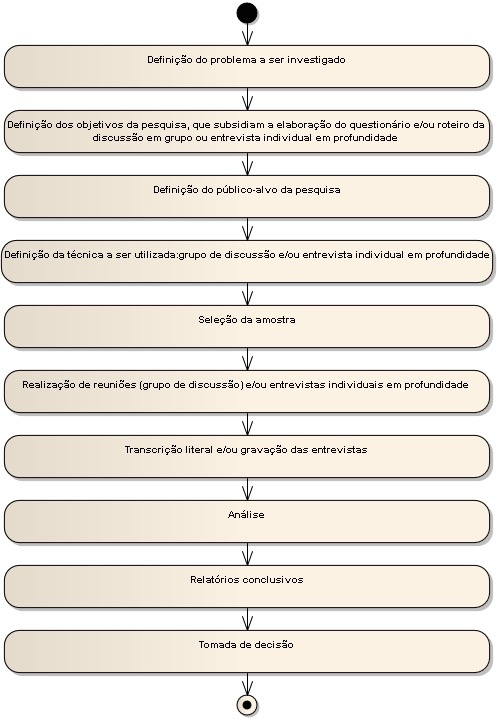
\includegraphics[scale=0.6]{figuras/fluxo_plan_questionario.jpg}
		\caption{Roteiro para elabora��o e aplica��o de uma pesquisa}
		\figsource{adaptado de 	\cite{manzato}}
		\label{Fig:fluxo:plan:quest}
	\end{figure}
}

\subsection{Planejamento e reda��o do question�rio}

Um fator muito importante neste ponto do processo era a necessidade de criar um question�rio pr�tico, simples de ser respondido e cujas respostas fossem geradas de forma imediata e sem necessidade de intera��o com terceiros (especialistas, por exemplo). Para tanto, decidiu-se por criar um question�rio digital que, em um primeiro momento foi confeccionado em uma planilha eletr�nica, podendo ser, posteriormente, transposto para um \sw ou p�gina de internet de forma simples e mantendo sua l�gica de funcionamento.

Para seguir o roteiro definido por \cite{manzato}, os objetivos que subsidiam a elabora��o do question�rio foram definidos como:

\begin{itemize}
	
	\item Coleta de dados sobre a situa��o atual da empresa em rela��o aos processos da \iso;
	
	\item Categoriza��o dos resultados de acordo com valores empresariais mais relevantes;
	
	\item Gera��o de uma lista de melhorias sugeridas ordenadas pelos valores empresariais.
	
\end{itemize}

\iftoggle{full}
{

	Al�m dos objetivos, o p�blico alvo da pesquisa tamb�m foi definido como pequenas empresas desenvolvedoras de \sw, chamadas de VSE \citep{iso}. Neste trabalho, somente a empresa alvo da disserta��o foi utilizada.

	A seguir ser� analisado como foi realizado o planejamento do question�rio.
}

\subsubsection{Classifica��o dos valores empresariais}

O primeiro passo foi a cria��o da classifica��o dos valores empresariais, cujo resultado pode ser observado na Figura \ref{Fig:class:valores}. Podemos notar tr�s estruturas principais: os valores empresariais na primeira coluna, as marca��es da classifica��o de import�ncia nas colunas seguintes e o c�lculo do peso final na �ltima coluna. Para simplificar a marca��o de import�ncia dos valores, foi colocado um guia visual na primeira linha que indica que as marca��es aumentam de valor da esquerda para a direita.

\iftoggle{full}
{
	
	O espa�o dispon�vel para as marca��es da classifica��o de import�ncia pode ser classificado como uma escala ordin�ria. Uma escala ordin�ria � composta por dados ordin�rios, ou seja, dados que podem ser ordenados \citep{garson}. No caso dos valores empresariais, a ordena��o � feita da esquerda para a direita, iniciando do mais importante para o menos importante. 

	O peso para cada valor empresarial � calculado de acordo com a marca��o de import�ncia e a quantidade de valores empresariais disponibilizados na pesquisa. No exemplo da Figura \ref{Fig:class:valores} � poss�vel observar 12 valores empresariais, sendo ``Comunica��o com o cliente'' o melhor classificado e, consequentemente, com o maior peso calculado e os valores ``Manuten��o e rastreabilidade entre artefatos'', ``Ger�ncia sobre o projeto como um todo'' e ``Ger�ncia de riscos'' os piores classificados e, consequentemente, com os menores pesos calculados.

}

\begin{figure}[!h]
	\centering
	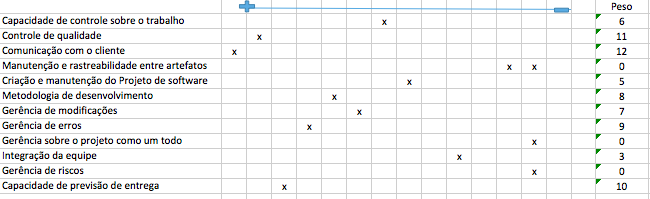
\includegraphics[scale=0.7]{figuras/class_valores.png}
	\caption{Classifica��o dos valores empresariais}
	\label{Fig:class:valores}
\end{figure}

A f�rmula para c�lculo do peso do valor empresarial, proposta por esta disserta��o, e o significado de seus termos est�o descritos na Tabela \ref{Tab:form:peso:valor}.

%$$p=n+1-c$$

%Onde \textit{p} � o peso, \textit{n} � a quantidade de valores empresariais dispon�veis e utilizados e \textit{c} � a coluna de classifica��o. Esta �ltima vari�vel possui um dom�nio de $1$ a $n+1$ para permitir que valores possam ter peso zero caso a coluna $n+1$ seja selecionada.

\begin{table}[h!]\footnotesize
	\centering
	\begin{tabular}
		{
			| >{\centering\arraybackslash}p{3cm}
			| >{\centering\arraybackslash}p{10cm}|
		}
		\hline
		
		\multicolumn{2}{|c|}{}\\
		\multicolumn{2}{|c|}{\large{$p=n+1-c$}}\\
		\multicolumn{2}{|c|}{}\\
		
		\hline
		
		\textbf{Vari�vel}&
		\textbf{Descri��o}\\
		\hline
		
		$p$&
		Peso do valor empresarial.\\
		
		\hline
		
		$n$&
		Quantidade de valores empresariais dispon�veis e utilizados.\\
		
		\hline
		
		$c$&
		Coluna de classifica��o. Possui um dom�nio de $1$ a $n+1$ para permitir que valores possam ter peso zero caso a coluna $n+1$ seja selecionada.\\
		
		\hline
		
	\end{tabular}
	\caption {F�rmula proposta para c�lculo do valor do peso empresarial}
	\label{Tab:form:peso:valor}
\end{table}


\subsubsection{Cria��o das perguntas}
\label{Sec:criacao:perguntas}

\iftoggle{full}
{

	O segundo passo foi a cria��o das perguntas que iriam compor o question�rio. Para tanto, foi necess�rio revisar a Norma \iso e extrair do seu conte�do o teor do que deveria ser averiguado das empresas candidatas � sua implanta��o para que o resultado refletisse os pontos fortes e fracos da organiza��o e que estes �ltimos fossem classificados de forma a fornecer um guia de inicializa��o da implanta��o.

	A Norma � dividida em duas �reas de conhecimento: \gp e \dsw. Cada �rea de conhecimento possui objetivos e processos que foram compilados a fim de estabelecer boas pr�ticas de desenvolvimento de \sw. Mais detalhes sobre as �reas de conhecimento, objetivos e processos se encontram na Se��o \ref{Sec:iso}.
	
	A estrat�gia de cria��o das perguntas seguida foi a leitura e interpreta��o de cada um dos processos da \iso. Ao se determinar a motiva��o e os objetivos de cada um dos processos, era necess�rio criar uma ou mais perguntas que avaliassem se a organiza��o pesquisada aplicava o processo e de que forma. Para uma avalia��o mais precisa, n�o era suficiente saber se a organiza��o possu�a e aplicava o processo e sim qual o n�vel de maturidade dela naquele processo espec�fico. Muitas vezes uma empresa poderia possuir um processo de distribui��o de tarefas, por exemplo, mas n�o possuir um plano de projeto e pap�is baseados neste plano para que essas tarefas fossem distru�das de acordo. Encontrar o n�vel de maturidade envolveria elaborar uma pergunta e distribuir as poss�veis respostas em uma escala que apontasse os diversos n�veis de maturidade impl�citos no processo.

	As perguntas foram elaboradas de forma fechada e com o objetivo de levar o pesquisado a refletir, buscar informa��es e avaliar sua organiza��o. As respostas, por sua vez, n�o conseguiriam abranger todas as possibilidades de maturidade e aplica��o do processo em quest�o. Uma forma de delimitar as possibilidades era utilizar uma escala de ranqueamento, que atribui valores de 1 a um dado valor m�ximo, geralmente 10, cujos limites s�o associados � percep��o do entrevistado em rela��o � pergunta, como ``concordo plenamente'' e ``discordo plenamente'' \citep{garson}. O problema com a escala de ranqueamento para este trabalho era como medir o n�vel de maturidade simplesmente informando dois extremos e possuindo um n�mero relativamente grande de subdivis�es entre eles. Essas subdivis�es, que representariam diferentes n�veis de percep��o da situa��o atual, poderiam levar o entrevistado a uma resposta ``pregui�osa'', onde ele n�o seria capaz ou n�o teria a disposi��o de raciocionar sobre sua situa��o atual. Ainda era poss�vel que o ranqueamento levasse a uma tend�ncia central de respostas, visto que o entrevistado tenderia a achar que a m�dia representaria melhor sua situa��o sem levar em considera��o pequenos fatores que desviariam a resposta para cima ou para baixo.

	A solu��o foi a escolha de uma escala de Likert adaptada, cuja forma tradicional utiliza itens de Likert como ``concordo plenamente'', ``concordo'', ``neutro'', ``discordo'' e ``discordo plenamente'', que tamb�m possuem valores associados como na escala de ranqueamento \citep{garson}. Por�m, caso se utilize a escala de Likert tradicional, os mesmos problemas da escala de ranqueamento acabariam por incindir nas respostas. Para melhores resultados, esses itens de Likert foram adaptados conforme as necessidades desta disserta��o: ao inv�s de itens gen�ricos, cada item descreveria o n�vel de maturidade dentro de sua escala, ou seja, cada pergunta possuiria cinco itens\footnotemark{} de Likert personalizados.

	\footnotetext{As escalas de Likert possuem, em geral, 4 ou 5 itens de Likert, sendo poss�vel encontrar um n�mero menor ou maior em situa��es espec�ficas.}
}

\iftoggle{full}
{
	A cria��o de cada item de Likert personalizado obedeceu ao seguinte processo:
}
{
	A cria��o das respostas obedeceu ao seguinte processo:
}

\begin{itemize}

	\item \textbf{Cria��o do item com maior valor na escala:} corresponderia a uma resposta que seria a transcri��o da defini��o do processo da Norma avaliado na pergunta, ou seja, o maior n�vel de maturidade de acordo com a Norma;
	
	\item \textbf{Cria��o do item com menor valor na escala:} a resposta que indicaria a contrapartida do item anterior, ou seja, o pior n�vel de maturidade, envolveria avaliar o cen�rio ideal e criar um cen�rio oposto ou conflitante com o primeiro e transcrev�-lo em forma de resposta � pergunta original;
	
	\item \textbf{Cria��o dos demais itens:} o processo anterior foi aproveitado para as demais respostas, incluindo elementos e situa��es que elevassem gradualmente o n�vel de maturidade do item de menor valor at� chegar pr�ximo ao item que representava o cen�rio ideal.
	
\end{itemize}	

\iftoggle{full}
{

	As respostas deveriam fazer com que o entrevistado pudesse encontrar uma situa��o na qual sua organiza��o melhor se encaixasse. Essa forma de cria��o das respostas levar�, em alguns momentos, o entrevistado a escolher entre duas op��es que n�o representam a sua realidade. Cabe a ele compreender que o ju�zo deve ser feito em termos relativos, escolhendo a resposta que mais se aproxima ao estado atual daquele processo.

	Esta forma de personaliza��o dos itens de Likert s�o propostas por esta  disserta��o como solu��o para um problema identificado na revis�o bibliogr�fica: ``As categorias de resposta nas escalas de Likert tem uma ordem de ranqueamento, mas os intervalos entre os valores n�o podem ser assumidos como iguais'' \citep{jamieson2004likert}. No artigo o autor diz que existem muitos n�veis entre um ``concordo plenamente'' e ``discordo plenamente'' que n�o podem ser quantificados em escalas equidistantes. Ao personalizar os itens trazendo mais significado para cada elemento, as dist�ncias das percep��es n�o s�o mais necessariamente iguais e a descri��o personalizada de cada elemento traz em si o n�vel de percep��o de valor que o pesquisador imaginou.
	
}

\subsubsection{Peso e \textit{score} da pergunta}

Aqui se encontra o cerne do processo, onde uma simples resposta com um valor em uma escala de Likert personalizada se transforma em um \textit{score} (pontua��o) dentro dos valores empresariais da empresa entrevistada.

Para tanto, o trabalho de constru��o de cada pergunta � finalizado com a atribui��o dos pesos relativos a cada valor empresarial identificado no in�cio do processo, conforme pode ser observado na Figura \ref{Fig:perg:peso}. Esses pesos quantificam o quanto aquele processo da \iso impacta ou � aderente ao valor empresarial. Na figura citada anteriormente, tr�s valores empresariais receberam os maiores pesos, o que significa que o processo avaliado tem fort�ssimo impacto sobre esses tr�s valores. Em contrapartida, 6 valores receberam peso zero, significando que n�o t�m influ�ncia alguma sobre o processo avaliado.

\begin{figure}[!h]
	\centering
	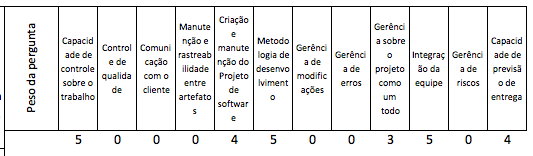
\includegraphics[scale=0.8]{figuras/pergunta_valor.png}
	\caption{Pesos dos valores de neg�cios das perguntas}
	\label{Fig:perg:peso}
\end{figure}

\iftoggle{full}
{

	A escala de valor que pode ser atribu�da ao peso da pergunta, diferentemente do peso dos valores que foram atribu�dos no in�cio do processo, pode assumir qualquer intervalo, pode ser discreta ou cont�nua e pode ser ajustada de acordo com a necessidade do entrevistado. Ela precisa obedecer somente a uma regra: deve ser escolhida com a mesma dire��o dos pesos dos valores de neg�cio, ou seja, se a ordena��o que se quer fazer � crescente, os valores devem ser crescentes. Na empresa alvo desta disserta��o foi escolhida uma escala crescente de 0 a 5.

	Assim como na elabora��o das respostas, foi necess�rio avaliar cada processo e cada pergunta em fun��o dos valores empresariais, realizando o ranqueamento de acordo com essa an�lise. Um outro avaliador poder� personalizar esses pesos de acordo com sua an�lise pessoal, tornando o resultado do question�rio mais condizente com sua realidade.

}

A f�rmula para c�lculo do \textit{score} final da pergunta, proposta por esta disserta��o, e o significado de seus termos est�o descritos na Tabela \ref{Tab:form:score}.

\begin{table}[h!]\footnotesize
	\centering
	\begin{tabular}
		{
			| >{\centering\arraybackslash}p{3cm}
			| >{\centering\arraybackslash}p{10cm}|
		}
		\hline
		
		\multicolumn{2}{|c|}{}\\
		\multicolumn{2}{|c|}{\large{$s_i=r \times v_i$}}\\
		\multicolumn{2}{|c|}{}\\
		
		\hline
		
		\textbf{Vari�vel}&
		\textbf{Descri��o}\\
		\hline
		
		$s$&
		\textit{Score} do valor empresarial.\\
		
		\hline
		
		$i$&
		Indica qual valor empresarial est� sendo calculado e varia de 1 ao n�mero total de valores.\\
		
		\hline
		
		$r$&
		Valor de Likert para a resposta selecionada.\\
		
		\hline
		
		$v$&
		Peso do valor empresarial $i$ associado aquela pergunta.\\
		
		\hline
		
	\end{tabular}
	\caption {F�rmula proposta para c�lculo do \textit{score} final da pergunta}
	\label{Tab:form:score}
\end{table}

%o \textit{score} final da pergunta ser� calculado de acordo com a seguinte f�rmula:

%$$s_i=r \times v_i$$

%Onde $s$ � o \textit{score} do valor empresarial $i$, $r$ � o valor de Likert para a resposta selecionada e $v$ � o peso do valor empresarial $i$ associado aquela pergunta. O �ndice $i$ indica qual valor empresarial est� sendo calculado e varia de 1 ao n�mero total de valores.

\iftoggle{full}
{

	O valor de Likert $r$ possui uma escala decrescente, inversa ao que seria intuitivo se imaginar. Isso se deve ao fato da primeira resposta representar o cen�rio ideal e, portanto, n�o precisar entrar na lista de melhorias que ser� sugerida como resultado final do question�rio. Isso signifca que \textit{scores} grandes representam processos que devem ser melhorados. Consequentemente, o inverso � verdadeiro: \textit{scores} pequenos ou zerados s�o processos que j� se encontram no n�vel ideal dentro da Norma \iso.

	Como pode ser observado no exemplo da Figura \ref{Fig:perg:score}, os tr�s valores que foram classificados com os maiores pesos no exemplo da Figura \ref{Fig:perg:peso} receberam os maiores \textit{scores} porque a resposta � pergunta foi o pior cen�rio poss�vel.

	Os �ltimos dois elementos presentes no \textit{score} por pergunta s�o: o maior \textit{score} e o \textit{score} total. Eles representam o resultado da avalia��o da pergunta e influenciam diretamente no objetivo final, que � a listagem ordenada das melhorias sugeridas.

	\begin{figure}[!h]
		\centering
		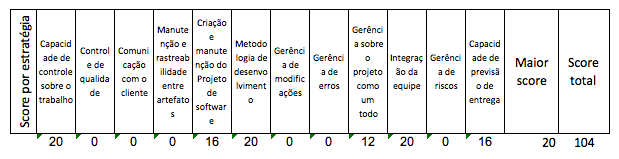
\includegraphics[scale=0.8]{figuras/pergunta_score.png}
		\caption{\textit{Scores} dos valores de neg�cios das perguntas}
		\label{Fig:perg:score}
	\end{figure}
	
}

\subsection{Realiza��o de campo}

\iftoggle{full}
{
	A defini��o da t�cnica a ser utilizada, pr�ximo passo do roteiro reproduzido na Figura \ref{Fig:fluxo:plan:quest}, foi limitada pelas caracter�sticas do question�rio. Por se tratar de um question�rio de auto avalia��o, a t�cnica a ser utilizada foi definida como entrevista individual, a ser conduzida pelo pr�prio pesquisado.

	N�o houve necessidade de sele��o da amostra, visto que o question�rio � individual, sendo a empresa alvo da disserta��o a �nica utilizada na pesquisa.
}

A aplica��o do question�rio pode ser dividida em duas etapas: revis�o e pontua��o dos valores empresariais e resposta �s perguntas. A seguir essas duas etapas ser�o descritas em mais detalhes.

\subsubsection{Revis�o e pontua��o dos valores empresariais}
\label{Sec:rev:pesos}

\iftoggle{full}
{

	O entrevistado deve revisar os valores empresariais sugeridos antes de come�ar o processo de pontua��o dos pesos. Caso o entrevistado n�o considere que os valores sugeridos sejam relevantes para a sua organiza��o, ou caso ele considere que outros valores devam ser adicionados, � importante que a lista de valores empresariais seja editada para refletir a realidade da organiza��o. 

	Pela primeira vers�o do question�rio ser uma planilha eletr�nica, esse tarefa de edi��o da lista de valores empresariais pode ser um pouco complexa e trabalhosa, visto que as f�rmulas n�o se ajustar�o automaticamente a mais colunas. Esse complicador ser� resolvido em vers�es futuras do question�rio que passar�o a ser constru�dos a partir de \sws e bancos de dados integrados.
}

De posse de todos os valores empresariais definidos e revisados, o entrevistado dever� iniciar o processo de atribuir os pesos. Por se tratar de uma classifica��o visual, como pode ser observado na Figura \ref{Fig:class:valores}, o processo � r�pido e bem simples.

\subsubsection{Resposta �s perguntas}

A fase final da aplica��o do question�rio consiste em respond�-lo de acordo com a realidade atual da empresa. Cada pergunta leva a uma lista de cinco poss�veis respostas que dever�o ser escolhidas de acordo com o texto que mais se aproxima da situa��o atual da organiza��o.

\iftoggle{full}
{
	Como j� mencionado na Se��o \ref{Sec:criacao:perguntas}, n�o � poss�vel descrever todas as possibilidades de cen�rio em apenas cinco respostas e a cria��o de uma amplitude maior de respostas tornaria o trabalho invi�vel. Portanto, o entrevistado dever� ter consci�ncia que sua escolha deve ser baseada no texto que mais se aproxima da sua realidade.

	O processo, apesar de ser longo pela grande quantidade de perguntas, se mostrou muito fluido e simples.
}

\subsection{Obten��o dos dados, an�lise e discuss�o dos resultados}
\label{Sec:resultados}

A avalia��o resultante das respostas obtidas no question�rio constr�i duas listas distintas com sugest�es de quais processos dever�o ser trabalhados prioritariamente. A primeira lista � composta pelos processos de \gp e a segunda pelos processos de \dsw. Ambas as listas s�o ordenadas pelo \textit{score} obtido a partir dos pesos dos valores empresariais e pela classifica��o do processo em rela��o � situa��o atual da empresa. � poss�vel observar os cinco primeiros processos de \gp na Figura \ref{Fig:resulado:PM} e os cinco primeiros processos de \dsw na Figura \ref{Fig:resulado:SI}.

\begin{figure}[!h]
	\centering
	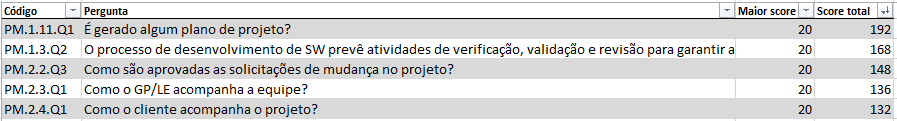
\includegraphics[scale=0.7]{figuras/resultado_PM.png}
	\caption{Resultados do question�rio (\gp)}
	\label{Fig:resulado:PM}
\end{figure}

\begin{figure}[!h]
	\centering
	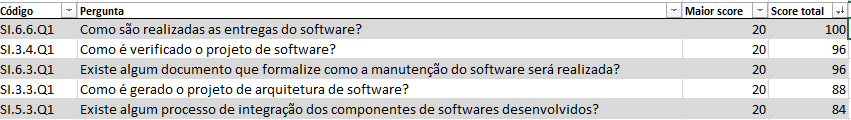
\includegraphics[scale=0.7]{figuras/resultado_SI.png}
	\caption{Resultados do question�rio (\dsw)}
	\label{Fig:resulado:SI}
\end{figure}

� dado ao entrevistado a op��o de ordenar a lista pelo maior \textit{score} ou pelo \textit{score} total. A diferen�a entre as duas ordena��es � que na primeira leva-se em considera��o o pior desempenho do processo dentre todos os valores empresariais dispon�veis e na segunda leva-se em considera��o o desempenho total do processo em todos os valores empresariais dispon�veis. Foi escolhida a segunda op��o de ordena��o nas duas listas.

Para cada elemento da lista, o entrevistado dever� se remeter ao texto original da pergunta para avaliar melhor o processo que dever� ser melhorado. No caso do primeiro processo da lista de \gp, conforme a Figura \ref{Fig:resulado:PM}, � necess�rio encontrar a pergunta codificada como ``PM.1.11.Q1''. O sistema de codifica��o das perguntas foi pensado para facilitar essa procura. O que o entrevistado ir� encontrar � o texto que pode ser observado na Figura \ref{Fig:perg:PM111Q1}.

	\begin{figure}[!h]
		\centering
		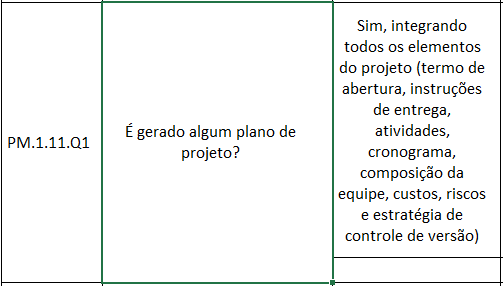
\includegraphics[scale=0.7]{figuras/pergunta_PM111Q1.png}
		\caption{Texto da pergunta classificada em primeiro lugar para \gp}
		\label{Fig:perg:PM111Q1}
	\end{figure}
	
A partir do texto original, o entrevistado dever� tra�ar seu plano de a��o para implantar melhorias que levem sua organiza��o ao cen�rio ideal, descrito na primeira op��o de resposta, tamb�m disponibilizada na Figura \ref{Fig:perg:PM111Q1}. Complementarmente, o entrevistado tamb�m pode se referenciar ao guia da \iso para encontrar mais detalhes das melhores pr�ticas para aplica��o do processo. Para facilitar esse procedimento, � disponibilizada no texto original da pergunta a nomenclatura do processo, como pode ser observado na Figura \ref{Fig:perg:PM111Q1_ISO}.

	\begin{figure}[!h]
		\centering
		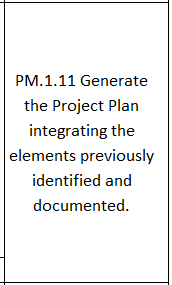
\includegraphics[scale=0.7]{figuras/pergunta_PM111Q1_ISO.png}
		\caption{Nomenclatura original do processo dentro do guia da \iso}
		\label{Fig:perg:PM111Q1_ISO}
	\end{figure}
	
Este processo de procura manual do texto original da pergunta para encontrar o cen�rio ideal e a refer�ncia do processo da \iso pode ser otimizado a partir de um \sw integrado que venha a substituir a planilha eletr�nica no futuro.

%\subsection{Projeto}

%O projeto foi a etapa onde as a��es necess�rias para a melhoria dos processos foram elencadas, priorizadas e devidamente documentadas. Tamb�m foram identificados os principais atores (\textit{stakeholders}), o cronograma, os recursos necess�rios e outros elementos, conforme diretrizes do PMBOK\footnotemark{} criado pelo PMI\footnotemark. Nesta etapa foram desenvolvidas as ferramentas de \sw que buscam facilitar as melhorias atrav�s da integra��o de informa��es vitais para os processos identificados.

%\footnotetext{\textit{Project Management Book Of Knowledge}, guia de boas pr�ticas de ger�ncia de projetos mundialmente reconhecido}
%\footnotetext{\textit{Project Management Institute}, institui��o internacional refer�ncia em ger�ncia de projetos.}

%\subsection{Conclus�o}

%A conclus�o consistiu na coleta dos resultados obtidos ap�s a implanta��o do projeto de melhoria dos processos e an�lise da qualidade destes resultados em compara��o ao cen�rio atual da empresa.

%\section{Estudo de caso}

%\subsubsection{Sele��o dos objetivos da \iso}
%\label{Sec:estr:obj:iso}
%
%Dentre os objetivos da \iso encontrados em \cite{iso}, foram selecionados 2 referentes � \gp e 1 referente ao \dsw. Podemos observar na Tabela \ref{Tab:estrat:obj:iso} a descri��o destes objetivos e a justificativa do porqu� foram selecionados.
%
%\begin{table}[h!]\footnotesize
%	\centering
%	\begin{tabular}
%		{
%			|p{7cm}
%			|p{7cm}|
%		}
%		
%		\hline
%		
%		\textbf{Objetivo \iso}&
%		\textbf{Problemas relacionados ao processo atual}\\
%		\hline
%		
%		PM.03 A \muda � abordada atrav�s de sua recep��o e an�lise. Mudan�as aos requisitos de \sw s�o avaliadas em custo, cronograma e impacto t�cnico.&
%		N�o existe processo formal para recep��o, an�lise e avalia��o da \muda.\\
%		\hline
%		
%		%	PM.O4 Reuni�es de revis�o s�o realizadas com a equipe de trabalho e o cliente. Acertos s�o registrados e rastreados.&
%		%	Reuni�es com o cliente n�o s�o registradas e os acertos s�o cadastrados no \sw Pend�ncias.\\
%		%	\hline
%		
%		PM.O6 Uma \vcs de \sw � desenvolvida. Itens da \swcfg s�o identificados, definidos e inclu�dos em uma \bline. Modifica��es e entregas de um item s�o controladas e disponibilizadas ao cliente e equipe de trabalho. O armazenamento, manuseio e entrega dos itens s�o controlados.&
%		Entregas de novas vers�es s�o realizadas sem nenhum controle de previs�o e aviso aos clientes.\\
%		\hline
%		
%		SI.O6 Uma \swcfg, que cumpra com o \req acertado com o cliente, que inclua documenta��es de usu�rio, opera��o e manuten��o � integrada, inclu�da na \bline e armazenada no \rep. Necessidades de mudan�a na \swcfg s�o detectadas e os pedidos de mudan�a relacionados s�o iniciados.&
%		N�o existe processo formal para recep��o, an�lise e avalia��o da \muda.\\
%		\hline
%		
%	\end{tabular}
%	\caption{Sele��o dos objetivos da \iso}
%	\label{Tab:estrat:obj:iso}
%\end{table}
%
%\subsubsection{Sele��o das atividades dos objetivos da \iso}
%
%
%Dentre as atividades que d�o suporte aos objetivos da \iso \cite{iso} selecionados em \ref{Sec:estr:obj:iso}, foram selecionadas as mais importantes e exequ�veis nesta primeira etapa de implanta��o dos processos na empresa objeto deste trabalho. As atividades selecionadas se encontram na Tabela \ref{Tab:estrat:ativ:iso}.
%
%As atividades iniciadas com a sigla PM s�o relacionadas � \gp e as iniciadas com a sigla SI ao \dsw.
%
%\begin{table}[h!]\footnotesize
%	\centering
%	\begin{tabular}
%		{
%			|p{7cm}
%			|p{3,5cm}
%			|p{3,5cm}|
%		}
%		
%		\hline
%		
%		\textbf{Atividade \iso}&
%		\textbf{Entradas}&
%		\textbf{Sa�das}\\
%		\hline
%		
%		PM.1.2 Definir com o Cliente as \entrega para cada um dos entreg�veis especificados na \dt.&
%		\dt (revisada)&
%		\ppj (\entrega)\\
%		\hline
%		
%		PM.1.4 Estabelecer a dura��o estimada para realizar cada tarefa.&
%		\ppj\par\begin{itemize}\item Tarefas\end{itemize}&
%		\ppj\par\begin{itemize}\item Dura��o estimada\end{itemize}\\
%		\hline
%		
%		PM.1.7 Atribuir datas estimadas de in�cio e t�rmino para cada uma das tarefas a fim de criar o \crono levando em considera��o os recursos, sequ�ncia e depend�ncias das tarefas.&
%		\ppj\par\begin{itemize}
%			\item Tarefas
%			\item Dura��o estimada
%			\item Composi��o da Equipe de Trabalho
%		\end{itemize}&
%		\ppj\par\begin{itemize}
%			\item \crono
%		\end{itemize}\\
%		\hline
%		
%		PM.2.2 Analisar e avaliar a \muda em rela��o ao custo, cronograma e impacto t�cnico. A mudan�a solicitada pode ser iniciada pelo cliente ou pela equipe interna de trabalho. Atualize o \ppj se as mudan�as aceitas n�o afetam acordos com o cliente. Solicita��es de mudan�a que afetem esses acordos devem ser negociadas por ambas as partes.&
%		\muda (iniciada)\par\ppj&
%		\muda (avaliada)\par\ppj (atualizado)\\
%		\hline
%		
%		PM.3.3 Identificar mudan�as aos requisitos e/ou \ppj relacionados � desvios significativos, riscos potenciais ou problemas relacionados � realiza��o do plano, documentando-os na \muda e acompanhando-os at� sua conclus�o.&
%		\prog (avaliado)\par&
%		\muda (iniciada)\\
%		\hline
%		
%		%	PM.3.2 Estabelecer a��es para corrigir desvios ou problemas e identificar riscos relacionados � realiza��o do \ppj, conforme necess�rio, documentando-os no \corre e acompanhando-os at� o seu fechamento.&
%		%	\prog (avaliado)\par&
%		%	\corre\\
%		%	\hline
%		
%		SI.6.6 Realizar entregas de acordo com as \entrega.&
%		\ppj\par
%		\begin{itemize}
%			\item \entrega
%		\end{itemize}\par
%		\swcfg&
%		\swcfg (entregue)\\
%		\hline
%		
%	\end{tabular}
%	\caption{Atividades da \iso}
%	\label{Tab:estrat:ativ:iso}
%\end{table}


%	Nesta se��o ser� apresentada a metodologia utilizada para a verifica��o das hip�teses apresentadas na Se��o \ref{hipoteses}.\\

%\subsection{Infraestrutura (Ambiente Real)}
%	Para execu��o dos testes foram criados e configurados 3 servidores com as seguintes especifica��es:
%	\begin{enumerate}
%		\item Processador Intel(R) Xeon(R) CPU X5650 2.67GHz (12 n�cleos)
%		\item 24 Gb de mem�ria RAM.
%		\item Disco R�gido SATA de 500 Gb.
%		\item Sistema Operacional Ubuntu Server 12.04.
%	\end{enumerate}
%	
%\subsection{Infraestrutura (Ambiente Virtual)}	
%	Em cada servidor real foram criados 3 servidores virtuais que foram instanciados simultaneamente para os testes. Estes servidores foram configurados da seguinte maneira:
%	\begin{enumerate}
%		\item QEMU Virtual CPU version 1.0 (Processador Intel(R) Xeon(R) CPU X5650 2.67GHz (12 n�cleos))
%		\item 4 Gb de mem�ria RAM.
%		\item Disco R�gido SATA de 10 Gb.
%		\item Sistema Operacional Ubuntu Server 12.04.
%	\end{enumerate}
%
%\subsection{Tipos de Testes de Concorr�ncia Executados}	
%	Todos os servidores compartilharam os recursos de processamento em seus 12 n�cleos para verificar a concorr�ncia das aplica��es. Os testes foram executados com as seguintes combina��es de ambientes:
%	
%	\begin{enumerate}
%		\item Ambiente Real;
%		\item Ambiente Virtual;
%		\item Ambiente Real X Ambiente Virtual;
%		\item Ambiente Virtual X Ambiente Real;
%		\item Ambiente Real X Ambiente Real;
%		\item Ambiente Virtual X Ambiente Virtual.
%	\end{enumerate}
%	
%	Para cada uma das combina��es acima foram executados 20 testes com os 4 algoritmos citados na Se��o \ref{dwarfs}, sendo computados os tempos de execu��o (individualmente e concorrentemente) e comparados os seus desempenhos. Os tempos de execu��o individuais foram utilizados como linha de base para a compara��o com os demais testes.\\
%

%\section{Abordagem do Problema}
%\label{abordagemDoProblema}
%	Para o planejamento dos testes tomou-se por base as conclus�es dos trabalhos apresentados na Se��o \ref{trabalhosrelacionados}. Entretanto como j� citado, estes trabalhos nos conduzem para a necessidade de obter informa��es sobre o efeito da concorr�ncia em ambientes compartilhados. Em toda a pesquisa realizada at� o momento, muito foi feito para avaliar o impacto de ambientes virtuais em servidores reais, mas nenhum destes estudos dedicou-se ao efeito da concorr�ncia causada pelas aplica��es executadas nestes ambientes, e a contribui��o do tipo de bibliotecas utilizadas na implementa��o destas aplica��es. \\
%	%quando � necess�rio o uso da concorr�ncia entre aplica��es. E at� o momento do encerramento do trabalho, n�o houve nenhuma abordagem que propusesse o uso do conceito de tipos de aplica��es para tratar este problema.
%	
%	E neste sentido, para que fosse poss�vel avaliar o efeito do compartilhamento foram testadas quatro tipos de aplica��es desenvolvidas com dois tipos de bibliotecas de programa��o paralela, OpenCL e OpenMP. As duas bibliotecas foram utilizadas por apresentarem boa documenta��o e por permitir testes de desempenho em diversas CPUs. Outro ponto importante � que esta abordagem permitiu o uso do Rod�nia, \textit{Benchmark} utilizado nos testes, que � apresentado na Se��o \ref{rodinia} e que possui implementa��o em OpenCL apresentado na Se��o \ref{opencl} e em OpenMP apresentado na Se��o \ref{openmp}.\\
%	
%	Os testes com as duas bibliotecas (OpenCL e OpenMP) se mostraram necess�rios devido �s diferen�as encontradas nos tempos de execu��o quando usadas em um mesmo algoritmo.\\
%	
%	Para os testes foram utilizados quatro \textit{Benchmarks} do Rod�nia que correspondem � tr�s tipos de classes. As classes de Dwarfs que foram escolhidas neste trabalho s�o: �lgebra Linear Densa (DLA), Grade Estruturada (SG) e Grafo Transversal (GT). A escolha por essas tr�s classes foi porque h� um grande n�mero de aplica��es cient�ficas em diversas �reas, como foi apresentado na Figura \ref{fig:dwarfs-areas} e em destaque na Figura \ref{fig:dwarfs-areas-destaque}. Al�m disso, o trabalho se concentra nestas tr�s classes porque abrangem o maior conjunto de tipos de aplica��es catalogadas pela abordagem dos Dwarfs.\\
%	
%	\begin{figure}
%		\centering\includegraphics[width=150mm]{Figuras/areasDwarfsDestaque.png}
%		\caption{Destaque das classes de Dwarfs usadas neste trabalho.}
%		\label{fig:dwarfs-areas-destaque}
%	\end{figure}
%
%\subsection{Classes e Algoritmos Escolhidos}
%	As seguintes classes de algoritmos foram escolhidos para testes de concorr�ncia:
%\begin{enumerate}
%	\item �lgebra Linear Densa � uma classe de Dwarf que envolve um conjunto de operadores matem�ticos realizados em valores escalares, vetores ou matrizes, quando a maioria dos elementos da matriz ou vetor s�o diferentes de zeros. Densa neste Dwarf refere-se � estrutura de dados aceita durante a computa��o. A intensidade aritm�tica do c�lculo operando os dados s�o de operadores de baixa intensidade (escalar por vetores, vetor-vetor, matriz-vetor , matriz-matriz, redu��o do vetor, vetor de digitaliza��o e produto escalar) que carregam um n�mero constante de opera��es aritm�ticas por elemento de dados. Tem uma raz�o elevada de opera��es matem�ticas para carga e um elevado grau de interdepend�ncia entre segmentos de dados. Eles s�o a base de solucionadores mais sofisticados, como LU de decomposi��o (LUD) ou Cholesky e apresentam alta intensidade aritm�tica \cite{Kaiser:2010}. Aplica��es classificados como DLA s�o relevantes atrav�s de uma variedade de dom�nios. Por exemplo, em ci�ncia dos materiais para a f�sica molecular e ci�ncia em nanoescala; em garantia de energia para a combust�o, fus�o e energia nuclear; na ci�ncia fundamental como astrof�sica e f�sica nuclear; no projeto de engenharia aerodin�mica. Algoritmos representativos desta classe s�o LUD, matriz transposta, matriz triangular, algoritmos de agrupamento, como K-means e Fluxo de cluster, e muitos outros. Os experimentos desta tese utilizou algoritmos LUD e Kmeans.\\
%	\begin{enumerate}
%		\item LUD � um algoritmo para calcular as solu��es de um conjunto de equa��es lineares que decomp�e a matriz como o produto de uma matriz triangular inferior e uma matriz triangular superior para conseguir uma forma triangular, que pode ser utilizada para resolver um sistema de equa��es lineares facilmente. A matriz $A \in$ $\mathbb{R}^{n \times n}$ tem uma fatora��o LU \emph{iff} todos os seus valores principais s�o n�o-zeros, ou seja, $det(A[1:k, 1:k]) \neq 0$ for $k = 1 : n-1$.\\
%		
%		\item Kmeans � um algoritmo de agrupamento amplamente utilizado na minera��o de dados, � um m�todo que particiona $n$ pontos que est�o em espa�o $d-$dimensional em $k$ aglomerados. O algoritmo semea $k$ aglomerados inicialmente no centro e determina para cada ponto de dados o seu centro mais pr�ximo, e ent�o recalcula os novos centros como o meio de seus pontos atribu�dos. Este processo de atribui��o de pontos de dados e reajustar centros � repetido at� que ele se estabilize.\\
%	\end{enumerate}
%	\item Grafo Transversal � um tipo de Dwarf que deve atravessar um n�mero de objetos em um gr�fico e examinar as caracter�sticas desses objetos. Um gr�fico ou uma rede s�o abstra��es intuitivas e �teis para a an�lise de dados relacionais, onde as entidades singulares s�o representadas como v�rtices, e as intera��es entre elas s�o retratadas como bordas. Aos v�rtices e �s bordas podem ser adicionalmente atribu�dos atributos com base na informa��o que encapsulam. Tais algoritmos normalmente envolvem uma quantidade significativa de mem�ria de acesso aleat�rio para pesquisas indiretas e pouca computa��o \cite{Kaiser:2010}. Dom�nios cient�ficos que incluem aplica��es importantes nesta classe s�o as de bioinform�tica (MUMmer), gr�ficos e pesquisa (BFS e B+Tree).\\
%	\begin{enumerate}
%		\item B+Tree � uma �rvore $n-$�ria muitas vezes com grande n�mero de filhos por n�. B+Tree consiste em uma raiz, n�s internos e folhas. A raiz pode ser uma folha ou um n� com dois ou mais filhos. O valor principal de uma B+Tree � no armazenamento de dados para recupera��o eficiente em um contexto de armazenamento orientados para o bloco. Isto se d� porque B+Tree tem alta ``fanout" (n�mero de apontadores para n�s filhos em um n�, tipicamente na ordem de 100 ou mais), o que reduz o n�mero de opera��es de E/S necess�rias para obter um elemento da �rvore. A ordem, ou fator de ramifica��o, b de uma B+Tree mede a capacidade de n�s (ou seja, o n�mero de n�s filhos) para n�s internos da �rvore. O n�mero real de filhos para um n�, referido aqui como m, � limitada para n�s internos de modo que $[b/2] \leq m \leq b$. N�s folha n�o tem filhos, mas s�o limitados, de modo que o n�mero de chaves deve ser de pelo menos $[b/2]$ e no m�ximo $b-1$. Na situa��o em que a B+Tree est� quase vazia, ela cont�m apenas um n�, que � um n� folha. A raiz � tamb�m a �nica folha, neste caso. A este n� � permitido ter uma chave, se necess�rio, e, no m�ximo, $b$ \\
%	\end{enumerate}
%	\item Grade Estruturada s�o algoritmos que servem para organizar dados em uma grade multidimensional regular, onde a computa��o se d� como uma s�rie de atualiza��es desta grade. Para cada atualiza��o da grade, todos os pontos s�o atualizados com valores a partir de uma pequena vizinhan�a em torno de cada ponto. A vizinhan�a est� normalmente impl�cita nos dados e determinada pelo algoritmo. Devido ao seu paralelismo inerente e calculo de natureza intensa, aplica��es de grade estruturados s�o geralmente uma boa op��o para as arquiteturas multi-core como GPU. Algoritmos de grade estruturada aparecem em muitos dom�nios cient�ficos que s�o citados a seguir com respectivo exemplo de aplica��o: imagens m�dicas (leuc�citos, Parede Cora��o e filtro de part�culas), simula��es de f�sica (\textit{HotSpot}), processamento de imagem (\textit{Speckle Reducing Anisotropic Diffusion}) e simula��es biol�gicas (mi�citos) \cite{Springer:2011}.\\
%	\begin{enumerate}
%		\item Speckle Reducing Anisotropic Diffusion (SRAD) � uma aplica��o de processamento de imagem para imagens de ultrassom e de radar. Ele reduz o ru�do de uma imagem dada, mantendo suas caracter�sticas importantes. Al�m disso, cada elemento da grade estruturada representa um pixel da imagem.\\
%	\end{enumerate}
%\end{enumerate}
%
%	
%\subsection{Ambiente de Testes}
%
%	O ambiente de testes necessita ser preciso afim de evitar que as avalia��es sejam prejudicadas. Para conseguir uma base funcional � necess�rio que o sistema seja ajustado seguindo algumas m�tricas de testes, tanto de hardware quanto de software e desta forma criou-se uma estrutura livre de testes tendenciosos.\\
%	
%	Para a an�lise de desempenho nos testes realizados foram colhidas 20 amostras, que se mostraram suficientes para gerar uma base de dados confi�vel. Este n�mero foi conseguido ap�s avaliar-se o intervalo de confian�a\footnote{C�lculo que apresenta o grau de confian�a de amostras estat�sticas.} das amostras. Neste caso foi avaliado que, desconsiderando aquelas com tempos constantes, as que mostravam varia��es de tempo de execu��o nas mesmas compara��es n�o eram significativas e ficavam em um intervalo pr�ximo com 10 execu��es. Assim, para se evitar conclus�es incertas, optou-se por testar 20 vezes cada combina��o de algoritmos, mesmo aquelas que possu�am tempos de execu��o constantes.\\
%	
%	Foram executados 4 tipos de algoritmos (B+Tree, Kmeans, LUD e SRAD) com combina��es de 2 tipos de bibliotecas (OpenMP e OpenCL) em ambientes reais e virtuais. Inicialmente foram testados os algoritmos em um ambiente livre de concorr�ncia para verificar os tempos de execu��o, afim de ter uma base de tempos para comparar a perda causada pela concorr�ncia em rela��o � n�o concorr�ncia. Comparou-se ent�o a concorr�ncia com todos os 4 algoritmos implementados usando a biblioteca OpenMP em ambientes reais e virtuais, seguido de todos os 4 algoritmos implementados em OpenCL em ambientes reais e virtuais (considerou-se estes testes como homog�neos) e por fim testou-se a concorr�ncia entre algoritmos implementados com as duas bibliotecas tamb�m executando a concorr�ncia em ambientes reais e virtuais (considerou-se estes testes como heterog�neos).\\
%	
%	Com todas as combina��es poss�veis e desconsiderando os testes iniciais de cada implementa��o, buscando a adequa��o dos testes, foram feitos 7120 testes, o que gerou uma base de conhecimento abrangente e confi�vel. Os resultados de todos estes testes s�o apresentados no Cap�tulo \ref{resultados}.\\
%%	Inicialmente foi feita uma an�lise gerencial de um ambiente na nuvem composto por recursos distintos em ambientes remotos, a fim de conseguir uma base de dados que possa ser utilizada pela Intelig�ncia Computacional (IC). Uma vez dispon�vel tal base, ser� poss�vel prever problemas em ambientes reais, j� que se poder� analisar que o evento que ocorreu anteriormente e que houve um problema associado a ele, ou mesmo que um conjunto de servidores/aplica��es n�o devem ser usados em conjunto, pois podem degradar o servi�o. De posse dessa an�lise, � poss�vel prever a ...

%\subsection{Defini��es e Metas dos Testes}

%		Este trabalho tem o foco principal no teste de desempenho, mediante avalia��o de tempo de execu��o quando h� concorr�ncia entre aplica��es para o mesmo recurso f�sico. Qualquer varia��o dos requisitos estipulados pelos testes deve ser tomada como uma n�o-conformidade e deve ser tratada desta forma. Este � o motivo desta se��o e fazem-se necess�rias as seguintes defini��es sobre testes:
%	
%	\begin{itemize}
%		\item Capacidade - � a carga de trabalho total que um sistema pode manipular sem violar os crit�rios de aceita��o.

%		\item Investiga��o - Busca o recolhimento de informa��es relacionadas com a velocidade, escalabilidade e/ou caracter�sticas de estabilidade do sistema. A avalia��o � frequentemente utilizada para provar ou refutar hip�teses sobre a causa de um ou mais problemas de desempenho observado.
%		
%		\item Lat�ncia - � uma medida da capacidade de resposta que representa o tempo que leva para completar a execu��o de um determinado processo. Pode-se tamb�m representar a soma de todas as lat�ncias de v�rios processos.
%		
%		\item M�tricas - S�o obtidas pela execu��o de testes de desempenho. As m�tricas normalmente s�o obtidos atrav�s de testes de desempenho, que incluem a utiliza��o do processador ou mem�ria ao longo de um determinado tempo.
%		
%		\item Desempenho - Refere-se a informa��es relativas ao tempo de resposta de uma aplica��o e/ou os n�veis de utiliza��o de recursos.
%		
%		\item Teste de Desempenho - � uma ``investiga��o" feita para determinar e/ou validar a velocidade, escalabilidade e/ou caracter�sticas de estabilidade do sistema. Este teste � o superconjunto que cont�m todas as outras subcategorias de testes de desempenho.


%		\item Teste de Unidade - � qualquer teste que visa as caracter�sticas de desempenho.
%		
%		\item Utiliza��o - � a porcentagem de tempo que um recurso est� ocupado. O percentual restante do tempo � considerado o tempo ocioso.

%	\end{itemize}

%\section{Normaliza��o dos Dados}
%\label{normal}
%	
%	A necessidade de normalizar os resultados se deu devido a an�lise dos tempos observados, que se mostraram, apesar de mesma grandeza (da ordem de segundos, ou no m�ximo minutos), serem diferentes quanto ao tempo de execu��o total, podendo um algoritmo executar em 50 segundos e outro em 8 minutos. Neste caso, houve a necessidade de executar o mesmo algoritmo (menor tempo de execu��o) diversas vezes para que houvesse concorr�ncia durante toda a execu��o do teste (algoritmo com execu��o mais longa). Com isso foi poss�vel extrair o percentual de aumento na execu��o concorrente do algoritmo de tempo mais longo e do algoritmo de tempo mais curto. Mas isto n�o foi suficiente para comparar individualmente cada algoritmo, sendo necess�rio criar um mecanismo que ``colocasse" todos os valores obtidos em uma mesma escala, e neste sentido optou-se pelo uso da normaliza��o de valores. Essa normaliza��o tem import�ncia para fornecer valores em uma escala pr�-definida que pode ser utilizada por escalonadores de tarefas para predizer o melhor recurso para executar determinado tipo de algoritmo, quando for necess�ria a exist�ncia de concorr�ncia.\\
%	
%	Para exemplificar melhor a normaliza��o de dados publicada por estes autores em \cite{licht:2013}, optou-se por apresentar recursos coletados de ordem de grandeza variadas em um n�vel onde os valores poder�o ser comparados mais facilmente, usou-se a F�rmula \ref{normalizacao}.\\
%\begin{equation}
%\label{normalizacao}
%	R = \frac{C - M2}{M1 - M2} (N1 - N2) + N2
%\end{equation}
%	Onde: \\
%	R : � o valor normalizado de cada entrada. \\
%	C : � o valor bruto coletado, sem tratamento. \\
%	M1 : � o maior valor encontrado em todos os valores lidos. \\
%	M2 : � o menor valor encontrado em todos os valores lidos. \\
%	N1 : � o maior valor da escala que se deseja trabalhar. \\
%	N2 : � o menor valor da escala que se deseja trabalhar. \\
%	
%	A maior vantagem do uso da F�rmula \ref{normalizacao} � poder elevar ou reduzir a pontua��o de tempos de acordo com a necessidade em cada medi��o e desta forma, j� que existe a compara��o entre todos os valores, a que tiver a maior pontua��o, � consequentemente a que tem a maior perda. Repara-se que o valor tratado de cada recurso poder� ser somado, j� que ap�s o uso da f�rmula, estar�o na mesma ordem de grandeza. Nesse exemplo, considera-se que os valores ter�o escala entre 0 e 9, sendo 0 para a menor perda de desempenho e 9 para a maior perda de desempenho.\\

%\begin{table}[h]
%\label{realnormal}
%\centering
%\caption{Tabela de Dados Reais Versus Dados Normalizados} % igual ao ambiente figura 
%\small
%\scriptsize
%\begin{tabular}{|c|c|c|c|c|c|c|c|c|c|c|c|c|c|}
%\hline
%\textbf{Algoritmo}  & \multicolumn{12}{c|}{\textbf{Tempo (segundos)}}                                 & \textbf{M�dia} \\ \hline
%Real B+Tree         & 14  & 14    & 14    & 14   & 14   & 14   & 14  & 14  & 14   & 14  & 14  & 14    & 14,05          \\ \hline
%V. B+Tree x V. SRAD & 221 & 218   & 220   & 223  & 219  & 219  & 221 & 225 & 223  & 217 & 221 & 218   & 220,6          \\ \hline
%R. B+Tree x V. LUD  & 21  & 21    & 22    & 20   & 20   & 21   & 21  & 22  & 21   & 21  & 21  & 21    & 21             \\ \hline
%V. B+Tree x R. SRAD & 211 & 214   & 212   & 216  & 212  & 213  & 215 & 211 & 213  & 214 & 211 & 214   & 213,1          \\ \hline
%\multicolumn{14}{|c|}{}                                                                                                \\ \hline
%\textbf{Algoritmo}  & \multicolumn{12}{c|}{\textbf{Tempo Normalizado}}                                & \textbf{M�dia} \\ \hline
%Real B+Tree         & 0   & 0     & 0     & 0    & 0    & 0    & 0   & 0   & 0    & 9   & 0   & 0     & 2,25           \\ \hline
%V. B+Tree x V. SRAD & 4,5 & 7,875 & 5,625 & 2,25 & 6,75 & 6,75 & 4,5 & 0   & 2,25 & 9   & 4,5 & 7,875 & 4,95           \\ \hline
%R. B+Tree x V. LUD  & 4,5 & 4,5   & 0     & 9    & 9    & 4,5  & 4,5 & 0   & 4,5  & 4,5 & 4,5 & 4,5   & 4,5            \\ \hline
%V. B+Tree x R. SRAD & 9   & 3,6   & 7,2   & 0    & 7,2  & 5,4  & 1,8 & 9   & 5,4  & 3,6 & 9   & 3,6   & 5,22           \\ \hline
%\end{tabular}
%\end{table}
%
%\begin{equation}
%\label{somatorio}
%	P = \frac{\sum _{k=1}^{r} x_{k}}{r} 
%\end{equation}
%	Onde: \\
%	P � a pontua��o obtida. \\
%	r � a quantidade de valores. \\
%	$x_{k}$ � cada recurso j� normalizado.\\
%	
%	Para verificar a aplica��o das f�rmulas foram tomadas 4 amostras de tempos de execu��o e a m�dia gerada por estes. � poss�vel comparar na Tabela 3.1 as 4 primeiras linhas os valores (em segundos) da execu��o de alguns algoritmos. Percebe-se, por exemplo, que a m�dia obtida por ``Real B+Tree" (14,05) tem uma ordem da valor bem menor que ``V. B+Tree x V. SRAD" (220,6), n�o podendo ser comparados diretamente, entretanto, ap�s normalizados, os valores aparecem como 2,25 e 4,95 respectivamente. Esta normaliza��o permite atribuir valores de forma que um escalonador poderia definir as melhores combina��es mediante uma escala de valores dentro de um intervalo pr�-definido, gerados pela F�rmula \ref{somatorio}.\\

%	Pode-se ainda, atrav�s da F�rmula \ref{somatorioComPesos} definir pesos para cada pontua��o afim de dar prioridade para determinadas combina��es, por exemplo, quando h� implementa��es com OpenMP e OpenCL (maior ou menor peso de acordo com o tipo de implementa��o).\\

%	As F�rmulas \ref{normalizacao}, \ref{somatorio} e \ref{somatorioComPesos} podem ainda ser utilizadas para outros tipos de dados, que referenciariam, capacidade de mem�ria, disco, cpu, ou qualquer outro tipo de valor de grandezas diferentes, por exemplo, para uma aplica��o que demanda maior quantidade de mem�ria, poder-se-ia atribuir um peso maior para servidores com mais mem�ria, esta entretanto � uma possibilidade a ser investigada em um novo projeto, n�o sendo contemplada por esta pesquisa.\\

%	\begin{equation}
%	\label{somatorioComPesos}
%		P = \frac{\sum _{k=1}^{r} x_{k} x p}{\sum_{k=1}^{r} p}
%	\end{equation}
%		Onde: \\
%		P � a pontua��o obtida por cada an�lise com os pesos de cada. \\
%		r � a quantidade de valores obtidos. \\
%		$x_{k}$ � cada valor j� normalizado.\\
%		p � o peso dado a cada item. \\


%	O uso da abordagem de normaliza��o definida aqui ser� melhor apresentada nos resultados da Se��o \ref{testesHeterogeneos}.

%\section{Conclus�o do Cap�tulo}
%	Este cap�tulo apresentou as metodologias utilizadas, bem como os testes efetuados afim de propor o conceito de afinidade e a avalia��o dos crit�rios de coexist�ncia de tipos de aplica��es. No pr�ximo cap�tulo ser�o apresentados os testes e os resultados obtidos � partir destas metodologias.


\chapter{An�lise dos resultados}
\label{analise:res}

Como p�de ser observado na Se��o \ref{Sec:resultados}, o resultado da auto avalia��o consiste em duas listas, uma para \gp e outra para \dsw, contendo as perguntas que foram classificadas como priorit�rias para um plano de a��o de melhorias. As Figuras \ref{Fig:resulado:PM} e \ref{Fig:resulado:SI} mostram os primeiros processos de ambas as listas, cuja ordena��o segue o \textit{score} calculado a partir dos valores empresariais e coloca nas primeiras posi��es os itens com pior desempenho.

A seguir ser�o analisados os cinco primeiros itens de cada lista com o intuito de validar o processo. Foram escolhidos somente dez elementos para an�lise pelo fato da lista ser muito extensa e tamb�m porque um plano de a��o para pequenas e m�dias empresas, segmento escolhido para ser tratado nesta disserta��o, tem maiores probabilidades de sucesso se executado em pequenas etapas e com um n�mero menor, e consequentemente mais gerenci�vel, de tarefas.

� importante frisar que as duas listas devem ser percorridas integralmente para se concretizar a implanta��o da \iso, principalmente se o objetivo final for a certifica��o na norma. Todos os processos e atividades que n�o satisfizerem os requisitos m�nimos dever�o ser abordados, fato que � facilitado pelos \textit{scores} gerados pelo processo criado por esta disserta��o.

Cada um dos dez itens ser� analisado frente aos tr�s principais valores empresariais do question�rio de auto avalia��o: comunica��o com o cliente, controle de qualidade e capacidade de previs�o de entrega.

\section{Itens priorizados de \gp}

\subsection{PM.1.11}

A pergunta ``� gerado algum plano de projeto?'' nos remete ao processo:

\begin{quote}
	``\textit{PM.1.11 Generate the Project Plan integrating the elements previously identified and documented}'' \citep{iso} - Gerar o plano de projeto integrando os elementos previamente identificados e documentados (tradu��o livre do autor).
\end{quote}	

O plano de projeto define como um projeto � executado, monitorado, controlado e encerrado \citep{pmbok}, se tornando um documento base para o seu gerenciamento. Sua influ�ncia nos principais valores empresariais pode ser observada nas an�lises a seguir:

\begin{description}
	
	\item[Comunica��o com o cliente:] o plano de projeto cont�m os planos de gerenciamento de comunica��o e das partes interessadas que, juntos, representam o planejamento da estrat�gia de comunica��o com todos os interessados pelo projeto, principalmente o cliente.
	
	\item[Controle de qualidade:] o plano de projeto cont�m os planos de gerenciamento da qualidade e outros planos subsidi�rios, tais como o plano de gerenciamento do escopo e requisitos, que oferecem os recursos necess�rios para garantir a qualidade dos sistemas desenvolvidos pela empresa.
	
	\item[Capacidade de previs�o e entrega:] o plano de projeto cont�m os planos de gerenciamento do tempo, escopo e requisitos, que possuem os elementos para controlar o trabalho e verificar se as tarefas necess�rias para a entrega dos produtos e servi�os est�o sendo realizadas dentro do cronograma, possibilitando prever atrasos antecipadamente.
	
\end{description}

Um plano de a��o que contenha este processo como primeiro item de trabalho trar� benef�cios relevantes para a organiza��o e observ�veis a curt�ssimo prazo. Por se tratar de base para a ger�ncia de projetos e endere�ar os tr�s principais valores empresariais da organiza��o alvo, por si s� j� seria um argumento que ratificaria o trabalho desta disserta��o.

A empresa alvo trabalha somente com uma Declara��o de Trabalho ou Termo de Abertura de Projeto que documentam as informa��es necess�rias para o in�cio do projeto mas n�o formalizam como o projeto ser� executado, monitorado, controlado e encerrado.

\subsection{PM.1.3}

A pergunta ``O processo de desenvolvimento de SW prev� atividades de verifica��o, valida��o e revis�o para garantir a qualidade do produto?'' nos remete ao processo:

\begin{quote}
	``\textit{PM.1.3 Identify the specific Tasks to be performed in order to produce the Deliverables and their Software Components identified in the Statement of Work. Include Tasks in the SI process along with verification, validation and reviews with Customer and Work}'' \citep{iso} - Identificar as tarefas espec�ficas que dever�o ser executadas para produzir as entregas e seus componentes de \sw identificados na Declara��o de Trabalho. Incluir tarefas no processo de \dsw junto com a verifica��o, valida��o e revis�o com o cliente (tradu��o livre do autor).
	
\end{quote}

A Declara��o de Trabalho � um dos primeiros documentos do projeto. Ele pode dar origem ou, dependendo do seu conte�do, ser considerado como o Termo de Abertura do Projeto. Este termo estabelece a parceria entre as empresas executora e requisitante do projeto \citep{pmbok} e origina as tarefas que produzir�o as entregas e componentes de \sw do projeto. Sua influ�ncia nos principais valores empresariais pode ser observada nas an�lises a seguir:

\begin{description}
	
	\item[Comunica��o com o cliente:] como pode ser observado na descri��o do processo, o cliente deve estar presente na cria��o, valida��o e revis�o das tarefas, evidenciando a import�ncia da comunica��o com o mesmo.
	
	\item[Controle de qualidade:] o processo de cria��o das tarefas prev� tamb�m a cria��o de crit�rios de aceita��o que ser�o utilizados em conjunto com os requisitos para a base do controle da qualidade.
	
	\item[Capacidade de previs�o e entrega:] a lista de tarefas originada pelo processo servir� de entrada para o processo de planejamento do tempo. De posse de uma lista completa, sem ambiguidades ou incoer�ncias, a empresa desenvolvedora ter� maior sucesso na estimativa do tempo de conclus�o do projeto.
	
\end{description}

Este processo trata diretamente da inclus�o do cliente no processo de \dsw, tornando a comunica��o com ele mais frequente e pr�xima. Assim como o item anterior, tamb�m cont�m elementos de grande influ�ncia nos outros principais valores empresariais. 

A emprea foco promove a inclus�o parcial do cliente neste processo. A Declara��o de Trabalho � enviada para o cliente para aprova��o mas n�o h� mais nenhum contato com o cliente no momento em que as tarefas originadas deste documento s�o validadas e verificadas, tornando esta melhoria um benef�cio observ�vel a curto prazo.

\subsection{PM 2.2}

A pergunta ``Como s�o aprovadas as solicita��es de mudan�a no projeto?'' nos remete ao processo:

\begin{quote}
	``\textit{PM 2.2 Analyse and evaluate the Change Request for cost, schedule and technical impact. The Change Request can be initiated externally by the Customer or internally by the Work Team. Update the Project Plan, if the accepted change does not affect agreements with Customer. Change Request, which affects those agreements, needs to be negotiated by both parties}'' \citep{iso} - Analise e avalie as solicita��es de mudan�a em fun��o dos impactos no custo, cronograma e elementos t�cnicos. As solicita��es de mudan�a podem ser inicializadas externamente pelo cliente ou internamente pela equipe de trabalho. Atualize o plano de projeto se a mudan�a aceita n�o afeta os acordos com o cliente. Solicita��es de mudan�a que afetem esses acordos precisam ser negociadas por ambas as partes. (tradu��o livre do autor).	
\end{quote}

As solicita��es de mudan�as propoem formalmente modifica��es em documentos, entregas ou linhas de base e podem resultar em atualiza��es em outras parte do plano de gerenciamento do projeto \citep{pmbok}. A influ�ncia deste processo nos principais valores empresariais pode ser observada nas an�lises a seguir:

\begin{description}
	
	\item[Comunica��o com o cliente:] al�m de tratar formalmente as solicita��es de mudan�as originadas pelo cliente, tamb�m atribui grande import�ncia na an�lise e avalia��o destas solicita��es. Mudan�as que afetem acordos previamente estabelecidos dever�o ser renegociadas com o cliente.
	
	\item[Controle de qualidade:] a an�lise e avalia��o das solicita��es de mudan�a contribuem para manter a coer�ncia entre o escopo e requisitos estabelecidos previamente.
	
	\item[Capacidade de previs�o e entrega:] um dos fatores que mais influenciam no atraso das entregas de um projeto � o aumento indiscriminado e n�o controlado do escopo. A an�lise e avalia��o das mudan�as estima necessidades de modifica��o do cronograma e at� mesmo a renegocia��o de prazos com o cliente.
	
\end{description}

Este processo abre um canal de comunica��o importante com o cliente, pois trata formalmente das mudan�as requisitadas no projeto e oferece procedimentos para duas situa��es que afetam diretamente o cliente: mudan�as iniciadas por ele e mudan�as que afetam acordos realizados com ele. 

Um dos principais fatores de descontentamento da empresa foco em seu processo produtivo � a falta de comunica��o com os clientes a respeito das suas solicita��es de mudan�a, tornando a melhoria neste processo um dos elementos mais importantes identificados neste trabalho.

\subsection{PM 2.3}

A pergunta ``Como o Gerente de Projetos/L�der de Equipe acompanha a equipe?'' nos remete ao processo:

\begin{quote}
	``\textit{PM.2.3 Conduct revision meetings with the Work Team, identify problems, review risk status, record agreements and track them to closure.}'' \citep{iso} - Conduzir reuni�es de revis�o com a equipe de trabalho identificando problemas, revisando status de riscos, registrando acordos e rastreando-os ao seu fechamento. (tradu��o livre do autor)
\end{quote}

As reuni�es s�o ferramentas utilizadas para discutir e endere�ar t�picos pertinentes ao projeto durante a execu��o e ger�ncia do seu trabalho \citep{pmbok}. A influ�ncia deste processo nos principais valores empresariais pode ser observada nas an�lises a seguir:

\begin{description}
	
	\item[Comunica��o com o cliente:] o processo em an�lise cita a reuni�o com a equipe de trabalho e n�o envolve o cliente diretamente.
	
	\item[Controle de qualidade:] as reuni�es s�o ferramentas muito eficientes, quando realizadas de forma correta, para acompanhar o trabalho e manter a qualidade dos produtos e servi�os, permitindo identificar n�o conformidades e tra�ar planos de a��o corretivos.
	
	\item[Capacidade de previs�o e entrega:] da mesma forma que citado no controle de qualidade, as reuni�es permitem detectar situa��es que possam levar ao atraso nas entregas e endere��-las a tempo de corrigir o rumo do projeto.
	
\end{description}

A empresa foco realiza reuni�es de acompanhamento com a equipe somente para projetos que apresentam problemas. A institui��o de reuni�es de acompanhamento trar�o benef�cios na qualidade do process de desenvolvimento de \sw e tamb�m na motiva��o da equipe, que passa a sentir mais valorizada no processo.

\subsection{PM 2.4}

A pergunta ``Como o cliente acompanha o projeto?'' nos remete ao processo:

\begin{quote}
	``\textit{PM.2.4 Conduct revision meetings with the Customer, record agreements and track them to closure. Change Request initiated by Customer or initiated by Work Team, which affects the Customer, needs to be negotiated to reach acceptance of both parties. If necessary, update the Project Plan according to new agreement with Customer.}'' \citep{iso} - Conduzir reuni�es de revis�o com o cliente, registrar acordos e rastre�-los ao seu fechamento. Requisi��es de mudan�a iniciadas pelo cliente, ou iniciadas pela equipe de trabalho mas que afetem o cliente, precisam ser negociadas para alcan�ar um acordo por ambas as partes. Se necess�rio, atualize o plano de projeto de acordo com os novos acordos com o cliente. (tradu��o livre do autor)
\end{quote}

As reuni�es foram definidas na an�lise anterior por�m a reuni�o deste processo em an�lise tem como principal foco o cliente e seu papel no controle do projeto. A influ�ncia deste processo nos principais valores empresariais pode ser observada nas an�lises a seguir:

\begin{description}
	
	\item[Comunica��o com o cliente:] um dos principais processos de inclus�o do cliente no processo de desenvolvimento de \sw, pois trata da revis�o do trabalho e endere�amento das solicita��es de mudan�as e poss�veis altera��es em acordos estabelecidos.
	
	\item[Controle de qualidade:] o processo de revis�o do trabalho com o cliente assegura que o projeto est� produzindo resultados de acordo com os crit�rios de qualidade estabelecidos pelo pr�prio cliente.
	
	\item[Capacidade de previs�o e entrega:] a revis�o do trabalho em conjunto com o cliente permite detectar situa��es que possam levar ao atraso nas entregas e endere��-las a em conjunto com o cliente a tempo de corrigir o rumo do projeto.
	
\end{description}

Este processo, assim como o PM.1.3, trata diretamente da inclus�o do cliente no processo de \dsw, tamb�m tornando a comunica��o com ele mais frequente e pr�xima. Assim como o item anterior, tamb�m cont�m elementos de grande influ�ncia nos outros principais valores empresariais. 

A empresa foco realiza reuni�es de acompanhamento com seus cliente somente em alguns projetos e em algumas poucas fases. A inclus�o do cliente em mais fases do projeto trar� benef�cios diretos em rela��o � confiabilidade e fideliza��o deste cliente.

\section{Itens priorizados de \dsw}

\subsection{SI.6.6}
\label{sec:si:entregas}

A pergunta ``Como s�o realizadas as entregas do software?'' nos remete ao processo:

\begin{quote}
	``\textit{SI.6.6 Perform  delivery  according  to Delivery Instructions}'' \citep{iso} - Realizar as entregas de acordo com as instru��es de entrega (tradu��o livre do autor).
\end{quote}	

O documento chamado de instru��es de entrega cont�m orienta��es de como \sw, relat�rios, documentos ou qualquer outro tipo de artefato do projeto dever�o ser entregues ao cliente. Ele deve ser parte integrante do \ppj e ser aprovado pelo cliente. A influ�ncia deste processo nos principais valores empresariais pode ser observada nas an�lises a seguir:

\begin{description}
	
	\item[Comunica��o com o cliente:] estabelece as condi��es e procedimentos para comunicar e realizar as entregas do projeto, colocando novamente o cliente como ator principal do processo.
	
	\item[Controle de qualidade:] a defini��o de como as entregas ser�o realizadas faz com que a qualidade seja inclu�da al�m do processo produtivo, visto que este passo final do processo � muitas vezes neglicenciado e levando a empresa desenvolvedora a cometer erros que poder�o manchar todo um trabalho bem feito e bem controlado em termos de qualidade.
	
	\item[Capacidade de previs�o e entrega:] junto com o acompanhamento do trabalho realizado, este � um dos principais processos que garantem a capacidade de previs�o e entrega.
	
\end{description}

Possuir este documento e executar o processo de acordo com as instru��es contidas no mesmo � pe�a fundamental para manter uma comunica��o eficiente com o cliente, adicionar qualidade ao projeto e garantir que tudo seja entregue dentro de sua previs�o.

Foi detectado que a empresa foco deste trabalho n�o possui instru��es de entrega formalizadas e isso causa conflitos com os clientes que n�o possuem previs�o de quando suas solicita��es ser�o atendidas. A implanta��o deste processo trar� benef�cios imediatos, aumentando a confiabilidade da empresa frente a seus clientes. 

\subsection{SI.3.4}
\label{sec:si:ver:proj:sw}

A pergunta ``Como � verificado o projeto de software?'' nos remete ao processo:

\begin{quote}
	``\textit{SI.3.4 Verify and obtain approval of the Software Design. Verify  correctness  of  Software  Design documentation,  its  feasibility  and  consistency with  their Requirement  Specification.  Verify  that the Traceability  Record contains the adequate relationships  between  requirements  and  the Software Design elements. The results found are documented  in  a  Verification  Results  and corrections  are  made  until  the document  is approved  by  DES.  If  significant  changes  were needed, initiate a Change Request.}'' \citep{iso} - Verificar e obter aprova��o do projeto de \sw. Verificar a corre��o da documenta��o de projeto de \sw, sua viabilidade e consist�ncia com as especifica��es de requisitos. Verificar se o registro de rastreabilidade cont�m os relacionamentos adequados entre requisitos e elmentos de projeto de \sw. Os resultados encontrados devem ser documentados em um documento de verifica��o de resultados e corre��es devem ser feitas at� o documento ser aprovado pelo analista. Se mudan�as significativas forem necess�rias, iniciar um pedido de mudan�a (tradu��o livre do autor).
\end{quote}	

O projeto de \sw � um documento que possui, entre outros elementos, os requisitos e a matriz de rastreabilidade, fundamentais para a constru��o do \sw. A influ�ncia deste processo nos principais valores empresariais pode ser observada nas an�lises a seguir:

\begin{description}
	
	\item[Comunica��o com o cliente:] revisar e aprovar o projeto de \sw � tamb�m um exerc�cio de revisar os requisitos do projeto que refletem, entre outras coisas, as necessidades do cliente. Em casos de incoer�ncia, ambiguidade ou falta de clareza, ser� necess�rio se comunicar com o cliente para garantir que os requisitos estejam corretos.
	
	\item[Controle de qualidade:] o processo em an�lise � fundamental para a qualidade do \sw, pois revisa os principais elementos para a sua constru��o.
	
	\item[Capacidade de previs�o e entrega:] para conseguir gerar uma previs�o de entrega � preciso que o trabalho n�o possua inconsist�ncias e todos os requisitos estejam corretos, tornando este processo essencial para a capacidade de previs�o de entrega.
	
\end{description}

A empresa foco deste trabalho n�o possui um processo formal de revis�o do projeto de \sw, levando muitos de seus projetos � entregas que n�o satisfazem as necessidades do cliente, expondo um controle de qualidade deficit�rio e gerando preju�zos por conta de retrabalhos e at� mesmo cancelamentos. Este processo contribuir� imediatamente para a melhoria no processo de desenvolvimento de \sw e tamb�m para a retomada da confiabilidade frente aos clientes.

\subsection{SI.6.3}

A pergunta ``Existe algum documento que formalize como a manuten��o do software ser� realizada?'' nos remete ao processo:

\begin{quote}
	``\textit{SI.6.4  Verify  and  obtain  approval  of  the Maintenance Documentation. Verify  consistency  of  Maintenance Documentation with Software Configuration. The  results  found  are  documented  in  a Verification  Results and  corrections  are  made until the document is approved by TL.}'' \citep{iso} - Verificar e obter aprova��o da documenta��o de manuten��o. Verificar a consist�ncia da documenta��o de manuten��o com a configura��o de \sw. Os resultados encontrados devem ser documentados em um documento de verifica��o de resultados e corre��es devem ser feitas at� o documento ser aprovado pelo l�de de equipe. (tradu��o livre do autor).
\end{quote}	

A documenta��o da manuten��o regula como o \sw ser� mantido ap�s sua entrega. Em alguns casos � um contrato formal entre a empresa desenvolvedora de \sw e o cliente. A influ�ncia deste processo nos principais valores empresariais pode ser observada nas an�lises a seguir:

\begin{description}
	
	\item[Comunica��o com o cliente:] o processo de verifica��o e aprova��o deve ser feito em conjunto com o cliente, principal interessado, incluindo mais uma vez o cliente no planejamento do projeto.
	
	\item[Controle de qualidade:] assim como citado na Se��o \ref{sec:si:entregas}, a qualidade deve estar presente al�m da execu��o do projeto e deve ser levada em considera��o na elabora��o da documenta��o de manuten��o.
	
	\item[Capacidade de previs�o e entrega:] n�o h� nenhuma rela��o com este valor empresarial, visto que as entregas j� ter�o sido realizadas quando a etapa de manuten��o estiver em vigor.
	
\end{description}

A empresa foco deste trabalho possui contratos formais de manuten��o dos seus \sw, mas n�o possui nenhum processo de verifica��o e aprova��o, principalmente um que inclua o cliente. Como consequ�ncia, alguns conflitos surgem ap�s a implanta��o do \sw e in�cio da fase de manuten��o. A ado��o deste processo trar� como benef�cio principal a participa��o e consequente valoriza��o do cliente no projeto.

\subsection{SI.3.3}

A pergunta ``Como � gerado o projeto de arquitetura de software?'' nos remete ao processo:

\begin{quote}
	``\textit{SI.3.3 Document or update the Software Design. Analyze  the  Requirements  Specification to generate  the  architectural  design,  its arrangement  in  subsystems  and  Software Components defining the internal and external interfaces.  Describe  in  detail,  the  appearance and the behaviour of the interface, based on the Requirements  Specification in a way that Resources for its implementation can be foreseen. Provide  the  detail  of Software  Components and their  interfaces  to  allow  the  construction  in  an evident way. Generate or update the Traceability Record.}'' \citep{iso} - Documente ou atualize o projeto de arquitetura do \sw. Analise as especifica��es de requisitos para gerar um projeto de arquitetura, seu arranjo em subsistemas e componentes de \sw definindo as interfaces internas e externas. Descreva em detalhes a apar�ncia e o comportamento das interfaces, baseado na especifica��o de requisitos de forma que os recursos necess�rios para sua implementa��o possam ser previstos. Provenha os detalhes de componentes de \sw e suas interfaces para permitir a constru��o de forma evidente. Gere ou atualize o registro de rastreabilidade. (tradu��o livre do autor).
\end{quote}	

O projeto de \sw foi discutido na Se��o \ref{sec:si:ver:proj:sw} e a influ�ncia deste processo nos principais valores empresariais pode ser observada nas an�lises a seguir:

\begin{description}
	
	\item[Comunica��o com o cliente:] a a��o de analisar os requisitos do projeto � equivalente a entender as necessidades do cliente. Em casos de incoer�ncia, ambiguidade ou falta de clareza, ser� necess�rio se comunicar com o cliente para garantir que os requisitos estejam corretos.
	
	\item[Controle de qualidade:] o processo em an�lise � fundamental para a qualidade do \sw, pois fornece os principais elementos para a sua constru��o.
	
	\item[Capacidade de previs�o e entrega:] para conseguir gerar uma previs�o de entrega � preciso que o trabalho n�o possua inconsist�ncias e todos os requisitos estejam corretos, tornando este processo essencial para a capacidade de previs�o de entrega.
	
\end{description}

Este processo tem um peso muito maior nos valores da qualidade e previs�o de entrega. Os documentos e a��es descritos acima fazem parte do ``centro nervoso'' do desenvolvimento de \sw: a arquitetura, que permite uma constru��o mais eficiente e integradas dos sistemas, melhor distribui��o do trabalho, reaproveitamento de componentes e escalabilidade (previs�o de crescimento do \sw). Por tratar e valorizar os requisitos, atinge indiretamente a comunica��o com o cliente, visto que estes devem ser levantados a partir de entrevistas e pesquisas realizadas em conjunto com o cliente.

A empresa foco n�o possui um processo formal de documenta��o do projeto de \sw. Assim como citado na Se��o \ref{sec:si:ver:proj:sw}, melhorias neste processo trar�o benef�cios imediatos como a retomada da confiabilidade dos clientes.

\subsection{SI.5.3}

A pergunta ``Existe algum processo de integra��o dos componentes de softwares desenvolvidos?'' nos remete ao processo:

\begin{quote}
	``\textit{SI.5.3  Integrates  the Software using Software Components and updates Test  Cases and Test Procedures for integration testing, as needed.}'' \citep{iso} - Integre o \sw utilizando componentes de \sw e atualize os casos e procedimentos de teste para testes de integra��o, conforme necess�rio. (tradu��o livre do autor).
\end{quote}	

A constru��o de um \sw a partir da integra��o dos seus componentes � uma pr�tica muito difundida e contribui para o desenvolvimento �gil de sistemas. A influ�ncia deste processo nos principais valores empresariais pode ser observada nas an�lises a seguir:

\begin{description}
	
	\item[Comunica��o com o cliente:] n�o h� relacionamento direto com este valor empresarial.
	
	\item[Controle de qualidade:] a modulariza��o na constru��o de um \sw permite que pequenos ``peda�os'' funcionais, tamb�m chamados de prot�tipos, possam ser entregues e validados pelo cliente, tornando o controle de qualidade uma atividade frequente durante o ciclo de vida do projeto. Os testes, citados no processo de integra��o, s�o considerados as principais ferramentas de controle de qualidade na �rea de desenvolvimento de \sw.
	
	\item[Capacidade de previs�o e entrega:] da mesma forma que citado anteriormente, a entrega de prot�tipos assegura que o projeto est� caminhando com sucesso ao seu objetivo e, caso contr�rio, permite identificar problemas a tempo de corrig�-los e manter a capacidade de realizar as entregas conforme combinado.
	
\end{description}

Este processo, assim como anterior, tem um peso muito maior nos valores da qualidade e previs�o de entrega, n�o tendo nenhum peso em rela��o � comunica��o com o cliente.

A empresa foco trabalha com a cria��o incremental de \sw, integrando componentes a cada etapa do projeto. Por�m, n�o possui um processo de testes bem definido, deixando o controle de qualidade deficit�rio. A melhoria na cria��o e aplica��o dos testes trar� benef�cios em termos de produtividade muito expressivos para a empresa.

\section{Resumo}

O resultado das an�lises realizadas anteriormente nos cinco processos de \gp e cinco processos de \dsw foi resumido na Tabela \ref{tab:resumo:analise}, que exibe os impactos de cada processo sugerido pela planilha de auto avalia��o nos tr�s principais valores empresariais.

\begin{table}[h!]\footnotesize
\centering
\begin{tabular}{|c|c|c|c|}
	\hline \textbf{Processo} & \textbf{Comunica��o com o cliente} & \textbf{Controle de qualidade} & \textbf{Capac.previs�o e entrega} \\ 
	\hline PM.1.11 & Alt�ssimo & Alt�ssimo & Alt�ssimo \\ 
	\hline PM.1.3 & Alt�ssimo & Alt�ssimo & Alto \\ 
	\hline PM.2.2 & Alt�ssimo & Alt�ssimo & Alt�ssimo \\ 
	\hline PM.2.3 & Nenhum & Alt�ssimo & Alt�ssimo \\ 
	\hline PM.2.4 & Alt�ssimo & Alt�ssimo & Alt�ssimo \\ 
	\hline SI.6.6 & Alt�ssimo & Alto & Alt�ssimo \\ 
	\hline SI.3.4 & M�dio & Alt�ssimo & Alto \\ 
	\hline SI.6.3 & Alto & M�dio & Nenhum \\ 
	\hline SI.3.3 & M�dio & Alt�ssimo & Alto \\ 
	\hline SI.5.3 & Nenhum & Alt�ssimo & Alto \\ 
	\hline 
\end{tabular} 
\caption {Impacto dos processos nos valores empresariais}
\label{tab:resumo:analise}
\end{table}
% % % % %\input{capitulo5.tex}
% % % % %\input{capitulo6.tex}
%\input{capitulo7.tex}
% % % % %\input{capitulo8.tex}
% !TEX root = dissertacao.tex
\chapter{Conclus�es}
	
\section{Considera��es Finais}

Os resultados obtidos no Cap�tulo \ref{Sec:resultados} geraram duas listas de processos priorizados pelos valores empresariais, sendo uma composta pelos processos de \gp e a outra pelos processos de \dsw. As Figuras \ref{Fig:resulado:PM} e \ref{Fig:resulado:SI} mostram os primeiros processos de ambas as listas.

A seguir ser�o analisadas as sugest�es de processos que dever�o ser trabalhados prioritariamente, sendo elencados os cinco primeiros elementos de cada lista.

\subsection{Itens priorizados de \gp}

\subsubsection{PM.1.11}

A pergunta ``� gerado algum plano de projeto?'' nos remete ao processo:

\begin{quote}
	``\textit{PM.1.11 Generate the Project Plan integrating the elements previously identified and documented}'' \citep{iso} - Gerar o plano de projeto integrando os elementos previamente identificados e documentados (tradu��o livre do autor).
\end{quote}	
 	
 
O plano de projeto � um documento base para o gerenciamento do projeto. Al�m de conter elementos que tratam da comunica��o com o cliente, tamb�m possui grande influ�ncia nos outros dois principais valores empresariais classificados como mais importantes: controle de qualidade e capacidade de previs�o e entrega. 
	
Um plano de a��o que contenha este processo como primeiro item de trabalho trar� benef�cios relevantes para a organiza��o e observ�veis a curt�ssimo prazo. Por se tratar de base para a ger�ncia de projetos e endere�ar os tr�s principais valores empresariais da organiza��o alvo, por si s� j� seria um argumento que ratificaria o trabalho desta disserta��o.

\subsubsection{PM.1.3}

A pergunta ``O processo de desenvolvimento de SW prev� atividades de verifica��o, valida��o e revis�o para garantir a qualidade do produto?'' nos remete ao processo:

\begin{quote}
	``\textit{PM.1.3 Identify the specific Tasks to be performed in order to produce the Deliverables and their Software Components identified in the Statement of Work. Include Tasks in the SI process along with verification, validation and reviews with Customer and Work}'' \citep{iso} - Identificar as tarefas espec�ficas que dever�o ser executadas para produzir as entregas e seus componentes de \sw identificados na Declara��o de Trabalho. Incluir tarefas no processo de \dsw junto com a verifica��o, valida��o e revis�o com o cliente (tradu��o livre do autor).
	
\end{quote}

Este processo trata diretamente da inclus�o do cliente no processo de \dsw, tornando a comunica��o com ele mais frequente e pr�xima. Assim como o item anterior, tamb�m cont�m elementos de grande influ�ncia nos outros principais valores empresariais. 

\subsubsection{PM 2.2}

A pergunta ``Como s�o aprovadas as solicita��es de mudan�a no projeto?'' nos remete ao processo:

\begin{quote}
	``\textit{PM 2.2 Analyse and evaluate the Change Request for cost, schedule and technical impact. The Change Request can be initiated externally by the Customer or internally by the Work Team. Update the Project Plan, if the accepted change does not affect agreements with Customer. Change Request, which affects those agreements, needs to be negotiated by both parties}'' \citep{iso} - Analise e avalie as requisi��es de mudan�a em fun��o dos impactos no custo, cronograma e elementos t�cnicos. As requisi��es de mudan�a podem ser inicializadas externamente pelo cliente ou internamente pela equipe de trabalho. Atualize o plano de projeto se a mudan�a aceita n�o afeta os acordos com o cliente. Requisi��es de mudan�a que afetem esses acordos precisam ser negociadas por ambas as partes. (tradu��o livre do autor).	
\end{quote}

Este processo abre um canal de comunica��o importante com o cliente, pois trata formalmente das mudan�as requisitadas no projeto e oferece procedimentos para duas situa��es que afetam diretamente o cliente: mudan�as iniciadas por ele e mudan�as que afetam acordos realizados com ele. Assim como o item anterior, tamb�m cont�m elementos de grande influ�ncia nos outros principais valores empresariais. 


\subsubsection{PM 2.3}

A pergunta ``Como o GP/LE acompanha a equipe?'' nos remete ao processo:

\begin{quote}
	``\textit{PM.2.3 Conduct revision meetings with the Work Team, identify problems, review risk status, record agreements and track them to closure.}'' \citep{iso} - Conduzir reuni�es de revis�o com a equipe de trabalho identificando problemas, revisando status de riscos, registrando acordos e rastreando-os ao seu fechamento. (tradu��o livre do autor)
\end{quote}

Este processo n�o cita diretamente o cliente mas possui elementos que est�o diretamente ligados � comunica��o com ele, como o registro de acordos que foi citado no item anterior. Este processo tamb�m cont�m elementos de grande influ�ncia nos outros principais valores empresariais. 

\subsubsection{PM 2.4}

A pergunta ``Como o cliente acompanha o projeto?'' nos remete ao processo:

\begin{quote}
	``\textit{PM.2.4 Conduct revision meetings with the Customer, record agreements and track them to closure. Change Request initiated by Customer or initiated by Work Team, which affects the Customer, needs to be negotiated to reach acceptance of both parties. If necessary, update the Project Plan according to new agreement with Customer.}'' \citep{iso} - Conduzir reuni�es de revis�o com o cliente, registrar acordos e rastre�-los ao seu fechamento. Requisi��es de mudan�a iniciadas pelo cliente, ou iniciadas pela equipe de trabalho mas que afetem o cliente, precisam ser negociadas para alcan�ar um acordo por ambas as partes. Se necess�rio, atualize o plano de projeto de acordo com os novos acordos com o cliente. (tradu��o livre do autor)
\end{quote}

Este processo, assim como o PM.1.3, trata diretamente da inclus�o do cliente no processo de \dsw, tamb�m tornando a comunica��o com ele mais frequente e pr�xima. Assim como o item anterior, tamb�m cont�m elementos de grande influ�ncia nos outros principais valores empresariais. 

\subsection{Itens priorizados de \dsw}

\subsection{Conclus�es}

Como pode ser observado nas Se��es anteriores, os resultados obtidos no Cap�tulo \ref{Sec:resultados} se mostraram muito satisfat�rios. A seguir ressalto algumas observa��es que resumem as an�lises feitas anteriormente:

\begin{itemize}
	
	\item Dentre os 5 primeiros itens priorizados para \gp, 3 est�o diretamente relacionados com o cliente (revis�o da qualidade do produto, aprova��o de solicita��es de mudan�as requisitadas pelo cliente e acompanhamento do projeto pelo cliente);
	
	\item Dentre os 5 primeiros itens priorizados para \dsw, 2 est�o diretamente relacionados com o cliente (entregas ao cliente e formaliza��o da manuten��o do \sw com o cliente);
	
	\item Os demais itens, das duas listas, est�o relacionados com processos que trar�o melhorias associadas indiretamente ao cliente.
	
\end{itemize}

\iftoggle{full}
{

	Esses n�meros indicam que, caso a organiza��o siga esta lista de prioriza��es e escolha os 5 primeiros itens para cada grupo, ela n�o somente ter� uma quantidade exequ�vel de a��es de melhorias de processos (10 processos em compara��o aos mais de 70 totais) como essas a��es iniciais ir�o abordar melhorias em �reas relevantes para a empresa ($50\%$ dos processos est�o ligados ao cliente, principal preocupa��o da organiza��o).

	Al�m disso, outros valores empresariais foram levados em considera��o nestas listas geradas pelo question�rio. Seus pesos influenciaram na prioriza��o e valores com pesos iguais ou pr�ximos ao atendimento ao cliente tamb�m posicionaram os processos associados no topo das listas.

	Levando em considera��o o objetivo desta disserta��o:
	\begin{quote}
		``Criar um m�todo de auto diagn�stico para implanta��o da \iso que priorize processos com maior ader�ncia aos valores individuais de cada empresa e que tragam benef�cios relevantes observ�veis nas etapas iniciais da implanta��o'' (Cap�tulo \ref{Sec:delim:trab})
	\end{quote} podemos afirmar que alcan�amos este objetivo.
	
}

A hip�tese levantada no Cap�tulo \ref{Sec:metodologia} afirmava que uma das melhores solu��es para o problema definido no Cap�tulo \ref{sec:def:prob} era a implanta��o de um question�rio de auto avalia��o. Analisando os resultados obtidos, podemos afirmar que o question�rio foi realmente uma ferramenta pr�tica e �til para a organiza��o montar sua estrat�gia de a��es de melhorias de processos.

\iftoggle{full}
{

	\section{Trabalhos Futuros}

	A fim de permitir uma maior flexibilidade na personaliza��o dos question�rios, o autor tem como meta futura transpor o question�rio de uma planilha eletr�nica para um \sw pr�prio. Conforme visto no Cap�tulo \ref{Sec:rev:pesos}, algumas dificuldades inerentes �s planilhas eletr�nicas tornam a tarefa de personaliza��o de alguns campos complexa e trabalhosa e um \sw aliado a um banco de dados trar�o benef�cios relevantes para este trabalho.

	Outro benef�cio da troca da planilha eletr�nica por um \sw espec�fico � a automa��o na procura pelo cen�rio ideal e refer�ncia � norma \iso para cada processo identificado na lista de melhorias. Pelas limita��es da planilha eletr�nica, o processo atual � manual e, consequentemente, exige mais tempo e trabalho do entrevistado. A partir de um \sw espec�fico integrado a um banco de dados, � poss�vel exibir o cen�rio ideal, nomenclatura original do processo na \iso e mais uma s�rie de informa��es, dicas e outras informa��es que auxiliem no planejamento e execu��o das melhorias. Ser� poss�vel realizar uma gest�o do conhecimento em cima dos processos, permitindo at� mesmo anexar documentos e refer�ncias externas para materiais de apoio. 

	Devido �s caracter�sticas do question�rio e das ideias de trabalhos futuros citadas anteriormente, uma solu��o desenhada para internet se mostra uma das melhores op��es. Al�m de maior disponibilidade, visto que o question�rio estaria dispon�vel em mais de um computador, tamb�m permite a utiliza��o de diferentes dispositivos, principalmente os m�veis como tablets e celulares.
	
}


%% !TEX root = dissertacao.tex

\appendix
\chapter{Casos de Uso}

\section{Atendimento}
\label{Sec:uc:atendimento}

\begin{figure}[!h]
\centering
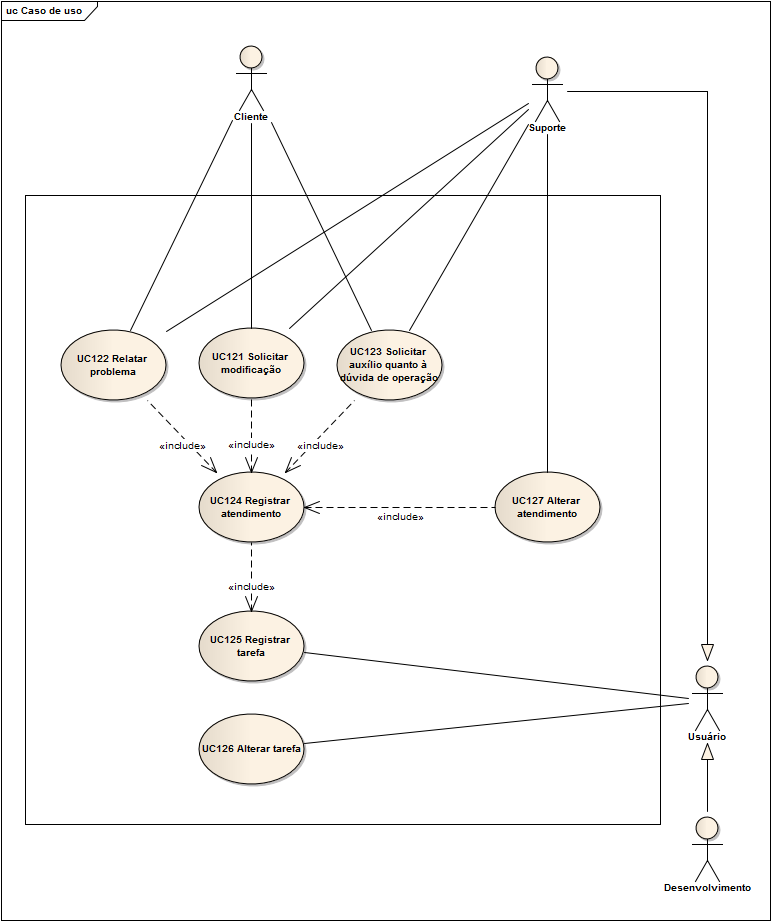
\includegraphics[scale=0.6]{figuras/UC_atendimento.png}
\caption{Caso de Uso: Atendimento}
\label{Fig:uc:atendimento}
\end{figure}

\subsection{Diagrama de Caso de Uso}

O diagrama est� representado na Figura \ref{Fig:uc:atendimento}.

\subsection{Atores}

\begin{itemize}

\item \textbf{Cliente:} cliente interno ou externo;
\item \textbf{Desenvolvimento:} pessoa respons�vel pelo desenvolvimento de sistemas;
\item \textbf{Suporte:} pessoa respons�vel pelo atendimento do departamento de Suporte T�cnico;
\item \textbf{Usu�rio:} usu�rio dos sistemas de atendimento, tarefas, etc.
 
\end{itemize}

\subsection{Descritivos dos Casos de Uso}

\subsubsection{UC121 Solicitar modifica��o}

\textbf{Principal - Solicitar modifica��o}

\begin{enumerate}
\item Cliente entra em contato para solicitar alguma modifica��o no sistema
\item Suporte registra o atendimento (UC124)
\item Suporte registra uma tarefa contendo a solicita��o para o Desenvolvimento (UC125)
\end{enumerate}

\subsubsection{UC122 Relatar problema}

\textbf{Principal - Relatar problema}

\begin{enumerate}
\item Cliente entra em contato para relatar algum problema
\item Suporte registra o atendimento (UC124)
\item \{Identificado erro no sistema\} Suporte registra uma tarefa contendo o erro do sistema para o Desenvolvimento (UC125)
\end{enumerate}

\subsubsection{UC123 Solicitar aux�lio quanto � d�vida de opera��o}

\textbf{Principal - Solicitar aux�lio}

\begin{enumerate}
\item Cliente entra em contato para solicitar aux�lio quanto � duvida de opera��o do sistema
\item Suporte registra o atendimento (UC124)
\end{enumerate}

\subsubsection{UC124 Registrar atendimento}

\textbf{Principal - Atendimento}

\begin{enumerate}
\item Suporte identifica o cliente no sistema de atendimento
\item Suporte categoriza o atendimento (d�vida, erro, solicita��o, etc.)
\item Suporte redige o texto que identifica os principais pontos do atendimento que foi efetuado
\item \{Atendimento conclu�do sem nenhuma pend�ncia\} Suporte fecha o atendimento
\item \{Atendimento conclu�do com alguma pend�ncia\} Suporte registra as tarefas referentes �s pend�ncias identificadas durante o atendimento
\end{enumerate}

\textbf{Alternativo - Cliente bloqueado}

\begin{enumerate}
\item O cliente identificado possui algum tipo de restri��o (inadimplente, bloqueado, etc.)
\item O sistema alerta:  "Cliente inadimplente/bloqueado"
\item Fim do caso de uso
\end{enumerate}

\textbf{Alternativo - Cliente n�o existe}

\begin{enumerate}
\item O cliente n�o foi identificado no sistema de atendimento
\item Sistema alerta  "Cliente n�o encontrado"
\item Fim do caso de uso
\end{enumerate}

\subsubsection{UC125 Registrar tarefa}

\textbf{Campos - Dados da tarefa}

\begin{itemize}
\item Respons�vel
\item Prioridade
\item Descri��o
\item Data limite para conclus�o
\item Data de previs�o
\item Data de conclus�o
\end{itemize}

\textbf{Principal - Registrar}

\begin{enumerate}
\item Usu�rio identifica respons�vel pela tarefa
\item Usu�rio preenche dados da tarefa
\item Usu�rio salva tarefa
\end{enumerate}

\subsubsection{UC126 Alterar tarefa}

\textbf{Principal - Alterar}

\begin{enumerate}
\item Usu�rio registra nova tarefa associada a uma tarefa j� existente
\item Usu�rio fecha uma tarefa atribu�da a ele
\end{enumerate}

\subsubsection{UC127 Alterar atendimento}

\textbf{Principal - Fechar}

\begin{enumerate}
\item Usu�rio fecha o atendimento
\end{enumerate}

\textbf{Principal - Novo registro}

\begin{enumerate}
\item Usu�rio inclui um novo registro a um atendimento j� cadastrado (n�o � permitido alterar o texto do atendimento j� cadastrado) (UC124)
\end{enumerate}

\textbf{Alternativo - Tarefas pendentes}

\begin{enumerate}
\item Usu�rio tenta fechar um atendimento que possua tarefas pendentes
\item Sistema alerta: "N�o � poss�vel fechar um atendimento com tarefas pendentes"
\end{enumerate}

% !TEX root = dissertacao.tex

\appendix
\chapter{Diagn�stico da empresa}

\subsection{An�lise Organizacional e de Processos}
\label{Sec:analise:org}

\textbf{Diagn�stico:} observou-se que a empresa possui qualidades essenciais para o crescimento cont�nuo, como por exemplo, o comprometimento dos profissionais, a comunica��o, o bom clima organizacional, assim como a cultura de prezar pela excel�ncia e ser reconhecida atrav�s da sua confiabilidade e qualidade nos servi�os. Por�m, para que a empresa suporte o crescimento que tende a acontecer cada vez mais, devido a demanda pelos servi�os, torna-se necess�rio alguns reajustes nos processos.

\subsubsection{Suporte T�cnico}
\label{Sec:suporte}

Este departamento � o �nico respons�vel pelo atendimento ao cliente atualmente. Os atendimentos podem ser realizados atrav�s do telefone, acesso remoto via internet, e-mail ou presencial. Como pode ser observado na Figura \ref{Fig:atend11}, somente 3 tipos foram registrados no m�s de novembro de 2014, mostrando que as comunicac�es via e-mail n�o s�o registradas.
%Assuntos sobre problemas e d�vidas relacionados aos \sws fornecidos s�o tratados diretamente com os t�cnicos do suporte. Para isso o departamento se utiliza de 2 \sws, cujas especifica��es est�o relacionadas na Tabela \ref{Tab:espec:sw:atend} e as janelas principais podem ser observadas nas Figuras \ref{Fig:jan:contatos:lanca} e \ref{Fig:jan:pendencias:lanca}.

%\begin{table}[h!]\footnotesize
%	\centering
%	\begin{tabular}
%		{
%			|p{1,5cm}|p{12cm}|
%		}
%		
%		\hline
%		\textbf{Nome}&
%		\textbf{Especifica��es}\\
%		\hline
%		
%		Contatos&
%		\begin{itemize}
%			\item Registra atendimentos;
%			\item Registra o cliente que est� sendo atendido;
%			\item Possui um espa�o virtualmente ilimitado para informar o assunto do contato;
%			\item Cronometra automaticamente o atendimento;
%			\item Possui uma data de previs�o de retorno;
%			\item N�o permite inclus�es de novas intera��es com o cliente durante o andamento do atendimento, que pode se estender por dias (neste caso novos atendimentos dever�o ser registrados, sem haver qualquer liga��o entre a primeira e as demais chamadas).
%		\end{itemize}\\
%		\hline
%		
%		Pend�ncias&
%		\begin{itemize}
%			\item Registra tarefas;
%			\item Registra o cliente que fez a solicita��o (opcional);
%			\item Associa o solicitante e o respons�vel por sua realiza��o (ambos colaboradores da empresa);
%			\item Permite definir prioridade, data limite para realiza��o e previs�o de atendimento;
%			\item Possui um controle de fechamento, onde o respons�vel indica a data em que aquela tarefa foi realizada;
%			\item Possui um controle de ``ok'', onde o solicitante indica que aquela tarefa j� foi liberada para o cliente;
%			\item Diferentemente do Contatos, permite acrescentar novas tarefas ao mesmo registro principal.
%		\end{itemize}\\
%		\hline
%		
%	\end{tabular}
%	\caption {Especifica��es dos \sws de atendimento}
%	\label{Tab:espec:sw:atend}
%\end{table}

%\begin{figure}[!h]
%	\centering
%	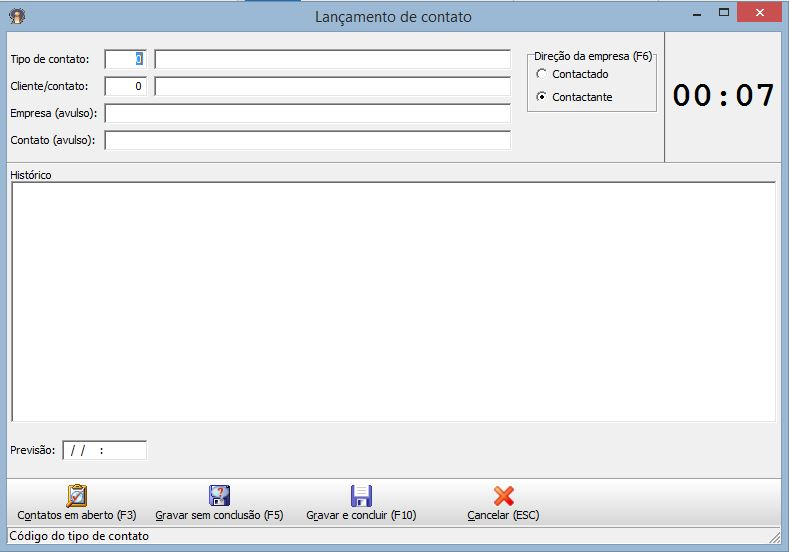
\includegraphics[scale=0.6]{figuras/jan_contatos_lancamento.jpg}
%	\caption{Janela de lan�amento dos atendimentos}
%	\label{Fig:jan:contatos:lanca}
%\end{figure}

%\begin{figure}[!h]
%	\centering
%	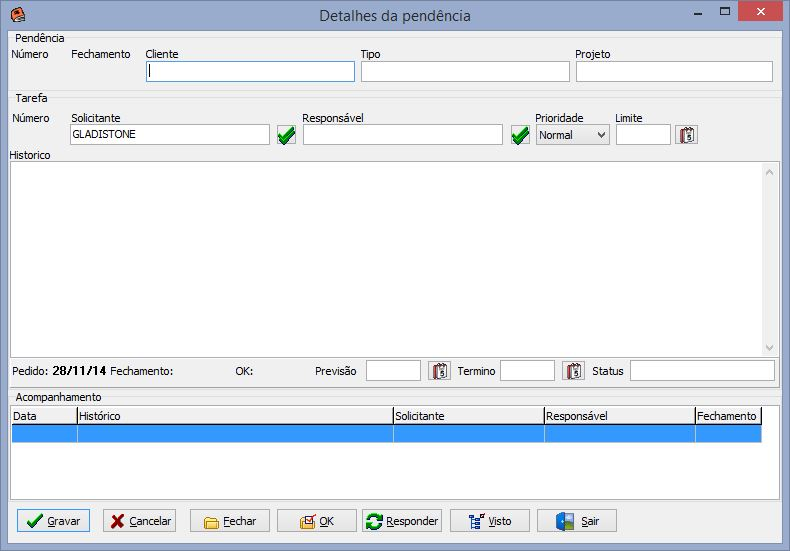
\includegraphics[scale=0.6]{figuras/jan_pendencias_lancamento.jpg}
%	\caption{Janela de lan�amento das pendencias}
%	\label{Fig:jan:pendencias:lanca}
%\end{figure}

\begin{figure}[!h]
	\centering
	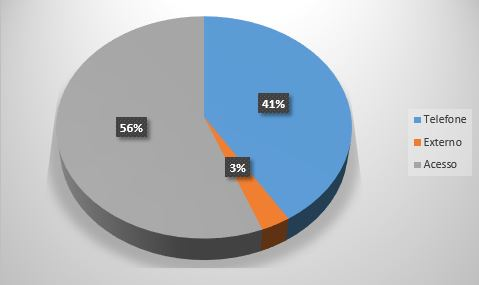
\includegraphics[scale=0.5]{figuras/atendimentos_por_tipo.jpg}
	\caption{Atendimentos por tipo em novembro/2014}
	\label{Fig:atend11}
\end{figure}

Outros problemas foram diagnosticados e est�o relacionados na Tabela \ref{Tab:probl:atend}, sendo a falta de acompanhamento do andamento das solicita��es e retorno ao cliente as mais cr�ticas.

\begin{table}[h!]\footnotesize
	\centering
	\begin{tabular}
		{
			|p{14cm}|
		}
		
		\hline
		\textbf{Problema diagnosticado}\\
		\hline
		
		Falta de registro de atendimento (para qualquer tipo)\\
		\hline
		
		Posterga��o de registro de atendimento (para qualquer tipo), que pode levar ao esquecimento (falta de registro)\\
		\hline
		
		Dados insuficientes sobre o contato\\
		\hline
		
		Falta de acompanhamento do andamento das solicita��es (fechamento dos registros de atendimento)\\
		\hline
		
		Falta de retorno da situa��o das solicita��es ao cliente\\
		\hline
		
		Tarefas originadas dos atendimentos, para o pr�prio departamento de suporte ou para outros departamentos, s�o registradas em um \sw separado e n�o h� nenhuma rastreabilidade\\
		\hline
		
	\end{tabular}
	\caption {Problemas diagnosticados no departamento de suporte}
	\label{Tab:probl:atend}
\end{table}

%As seguintes a��es devem ser tomadas para contonar os problemas diagnosticados:
%
%\begin{itemize}
%	
%	\item Todos os chamados t�cnicos dever�o ser registrados no ato de sua execu��o (liga��o, acesso remoto ou recebimento do e-mail), com exce��o do atendimento externo que deve ser registrado no ato do retorno do t�cnico;
%	
%	\item O m�ximo de informa��es poss�veis precisa ser registrado no hist�rico do chamado;
%	
%	\item A fus�o entre o Contatos e o Pend�ncias � extremamente necess�ria, a fim de criar um registro de todas as a��es vinculadas naquele chamado, tornando-se obrigat�rio o registro de todas as a��es realizadas por cada t�cnico que atender o chamado;
%	
%	\item Qualquer nova informa��o de um chamado deve ser adicionada ao registro j� aberto, sem a necessidade de abrir um novo chamado e permitindo a rastreabilidade;
%	
%	\item Um departamento de Servi�o de Atendimento ao Cliente (SAC) dever� ser criado e pelo menos uma pessoa deve ser colocada como respons�vel pelas suas atribui��es;
%	
%	\item O SAC realizar� o fechamento do chamado junto ao cliente, consultando se realmente o problema foi solucionado e realizando pesquisas de satisfa��o e gerando indicadores de desempenho e qualidade (tempo m�dio de conclus�o dos chamados, problemas mais ocorridos, cliente mais ativo, t�cnico mais ativo, etc);
%	
%	\item Os clientes dever�o receber um Documento de Abertura e Acompanhamento de Chamados, juntamente com o manual  do \sw, para que saibam exatamente como proceder para abrir e acompanhar um chamado;
%	
%	\item Para uma melhor performance da equipe de suporte, dever� ser feito a gest�o do conhecimento, documentando a resolu��o de cada problema que surja no atendimento do suporte t�cnico;
%	
%	\item � necess�ria a elabora��o de um fluxograma do atendimento, com as informa��es chaves de requisitos para abertura de chamados;
%	
%	\item � necess�ria a elabora��o de um fluxograma do atendimento de servi�os diferenciados, tais como treinamentos, suportes avulsos, entrada de equipamento para concerto ou manuten��o, entre outros, lembrando de acrescentar no fluxo a emiss�o da Ordem de Servi�o;
%	
%	\item Dever� ser realizado o acompanhamento dos clientes que n�o abrem chamado com o suporte h� mais de 3 meses.
%	
%\end{itemize}

\subsubsection{Desenvolvimento}
\label{Sec:desenvolvimento}

Este departamento n�o tem contato direto com os clientes, pois todas as solicita��es passam pelo departamento de suporte t�cnico. Por�m, todas as solcita��es de mudan�a ou corre��o de problemas nos \sws s�o resolvidas por este departamento e alguns atendimentos s�o repassados para o setor de desenvolvimento para resolu��o conjunta quando os t�cnicos n�o possuem conhecimento ou capacidade para trat�-los por si mesmos.

Os problemas diagnosticados para este departamento est�o relacionados na Tabela \ref{Tab:probl:desenv}.

%As tarefas deste departamento s�o registradas no \sw Pend�ncias mas, como j� relatado anteriormente, n�o possuem relacionamento com os chamados abertos no \sw Contatos. 

\begin{table}[h!]\footnotesize
	\centering
	\begin{tabular}
		{
			|p{14cm}|
		}
		
		\hline
		\textbf{Problema diagnosticado}\\
		\hline
		
		Falta de posicionamento quanto ao andamento das solicita��es\\
		\hline
		
		Falta de previs�o de entrega das solu��es\\
		\hline
		
		Falta de rastreabilidade entre abertura de chamados e tarefas\\
		\hline
		
	\end{tabular}
	\caption {Problemas diagnosticados no departamento de desenvolvimento}
	\label{Tab:probl:desenv}
\end{table}

%Para solucionar os problemas diagnosticados para este setor, al�m das a��es ja citadas em \ref{Sec:suporte}, ser�o necess�rias as seguintes a��es:
%
%\begin{itemize}
%	
%	\item Criar processos para determinar a previs�o de lan�amento de vers�es de \sws;
%	
%	\item Criar processos para determinar em qual vers�o determinada solicita��o ser� inclu�da;
%	
%	\item Integrar aos \sws de atendimento as informa��es de lan�amento de vers�es e, consequentemente, a previs�o das solicitac�es.
%	
%\end{itemize}

\subsubsection{Financeiro}

O departamento financeiro lida com o cliente com uma frequ�ncia menor que os departamentos de suporte e desenvolvimento. Por�m, os assuntos relacionados a este departamento podem gerar transtornos e preju�zos quando feitos de forma incorreta. Al�m disso, este departamento tamb�m � respons�vel por bloquear o atendimento aos clientes inadimplentes, portanto representa um papel importante nos processos descritos em \ref{Sec:suporte} e \ref{Sec:desenvolvimento}.

O principal problema detectado neste departamento foi a falta de registro dos contatos realizados com o cliente.

%Nenhum atendimento ou tarefa relacionados a este departamento s�o registrados nos \sws de atendimento. Portanto, as a��es necess�rias para melhoria dos processos s�o:

%\begin{itemize}
%	
%	\item Registrar todo e qualquer contato com clientes nos \sws de atendimento;
%	
%	\item Integrar as informa��es financeiras com os \sws de atendimento para que a libera��o ou bloqueio seja feito automaticamente no ato da identifica��o do cliente.
%	
%\end{itemize}

\subsubsection{Marketing}

O departamento de marketing � o respons�vel, geralmente, pelo primeiro contato com o cliente. Durante as negocia��es de venda de \sw, � comum haver solicita��es de modifica��es ou acertos sobre configura��es, convers�es de dados e treinamentos. %Por�m, nenhuma dessas informa��es s�o registradas nos \sws de atendimento. O mesmo ocorre na venda de equipamentos e outros servi�os.

O principal problema detectado neste departamento foi a falta de registro dos contatos realizados com o cliente.

%Portanto, as a��es necess�rias para melhoria dos processos s�o:
%
%\begin{itemize}
%	
%	\item Registrar os primeiros contatos com todos os prospectos, mesmo que n�o se tornem clientes;
%	
%	\item Registrar toda e qualquer intera��o com os clientes, novos ou antigos;
%	
%	\item Incluir nos registros as informa��es sobre negocia��o, poss�veis modifica��es, convers�es e outras condi��es estabelecidas durante ou ap�s a venda.
%	 
%\end{itemize}

\subsection{An�lise SWOT}

A fim de resumir e melhor entender a an�lise organizacional e de processos realizada em \ref{Sec:analise:org}, foi desenvolvida a Tabela \ref{Tab:SWOT} com a an�lise SWOT.

\begin{table}[h!]\footnotesize
\centering
\begin{tabular}
{
	| >{\centering\arraybackslash}p{7cm}
	| >{\centering\arraybackslash}p{7cm}|
}
\hline

	For�as&
	Fraquezas\\
	\hline

	%For�as
	\begin{tabular}{p{6,8cm}}
	Comprometimento dos profissionais;\\
	Bom clima organizacional;\\
	Cultura de prezar pela excel�ncia;\\
	Ser reconhecida atrav�s da sua confiabilidade e qualidade nos servi�os.\\
	\end{tabular}&

	%Fraquezas
	\begin{tabular}{p{6,8cm}}
	Falta de informa��es no acompanhamento de solicita��es;\\
	Inefici�ncia na comunica��o com o cliente.\\
	\end{tabular}\\
	\hline

	Oportunidades&
	Amea�as\\
	\hline

	% Oportunidades
	\begin{tabular}{p{6,8cm}}
	Taxa de crescimento elevada nos �ltimos meses;\\
	Aumento no faturamento;\\
	Alta divulga��o da marca, dentro e fora da sua pr�pria cidade.\\
	\end{tabular}&

	% Amea�as
	\begin{tabular}{p{6,8cm}}
	Perder a confiabilidade dos clientes;\\
	Manchar a reputa��o;\\
	Sofrer queda nas vendas pela perda de indica��es de clientes e parceiros insatisfeitos;\\
	Sofrer perda de clientes j� estabelecidos por n�o prestar um bom atendimento.\\
	\end{tabular}\\
	\hline

\end{tabular}
\caption {An�lise SWOT dos processos}
\label{Tab:SWOT}
\end{table}


%\subsection{Estrat�gia}
%
%\label{Sec:ec:estrategia}
%
%A implanta��o de um novo processo, ou de sua melhoria, � uma atividade que possui um custo financeiro, de tempo e de recursos muito alto para qualquer empresa, independente do seu porte. A implanta��o de processos baseados em normas pode ser ainda mais custoso e complexo, principalmente para uma pequena empresa.
%
%Por conta destes fatores, a empresa objeto de estudo desta disserta��o optou por realizar a implanta��o incremental da \iso, escolhendo as �reas mais deficientes citadas no diagn�stico que se encontra no Cap�tulo \ref{Cap:analise:cenario}.
%
%Esta disserta��o teve como foco o tratamento dos problemas identificados no departamento de \textbf{Desenvolvimento}, descritos na Se��o \ref{Sec:desenvolvimento}. Apesar do foco ter sido em somente um departamento, foi observado que as solu��es propostas afetariam diretamente os demais departamentos, pois havia uma raiz comum a todos os problemas diagnosticados: a comunica��o com o cliente. A cria��o de processos bem estruturados de registro de atendimentos em conjunto com ferramentas que suportassem estes processos cobririam todos os problemas diagnosticados.
%
%Outro fato de suma import�ncia observado foi a abrang�ncia da solu��o proposta. Apesar do estudo de caso ter sido feito em uma empresa de desenvolvimento de \sw, outros segmentos podem se beneficiar do processo de integra��o entre registro de contato com o cliente e controle de tarefas. 
%
%Para se alcan�ar o objetivo desta disserta��o, foi adotada como estrat�gia inicial a sele��o dos objetivos da \iso, descritos nas Se��es \ref{Sec:iso:obj:gp} e \ref{Sec:iso:obj:dsw}, que pudessem contribuir para a solu��o dos problemas identificados na an�lise realizada no Cap�tulo \ref{Cap:analise:cenario}.
%
%Ap�s a sele��o e an�lise dos objetivos da \iso, foram relacionadas as atividades mais importantes de cada um destes objetivos que dariam suporte ao alcance dos objetivos deste trabalho.
%


%\bibliographystyle{brazil}
\bibliography{research}
\bibliographystyle{Bibliografia/apalike-pt}     
% utilize macros (3 primeiras letras do mes em ingles, minusculas) no seu
% .bib para atribuir o nome do mes em portugues nas referencia,
% se o style for brazil, outros estilos tambem aceitam estas macros
% Ex:
%
% @InProceedings{teste,
%   author =       {Luciano}
%   year =         {2000}
%   month =        {}#sep;
% }
%
\addcontentsline{toc}{chapter}{\MakeUppercase{Bibliografia}}

\singlespacing
\makecapadissertacao

\end{document}
